\chapter{L’Equateur de Baños à Quito}
\section*{29 juin 2015}
Je quitte Baños par la route des cascades qui descend vers l'Amazonie sur 60km. \newline
 \newline
\centerline{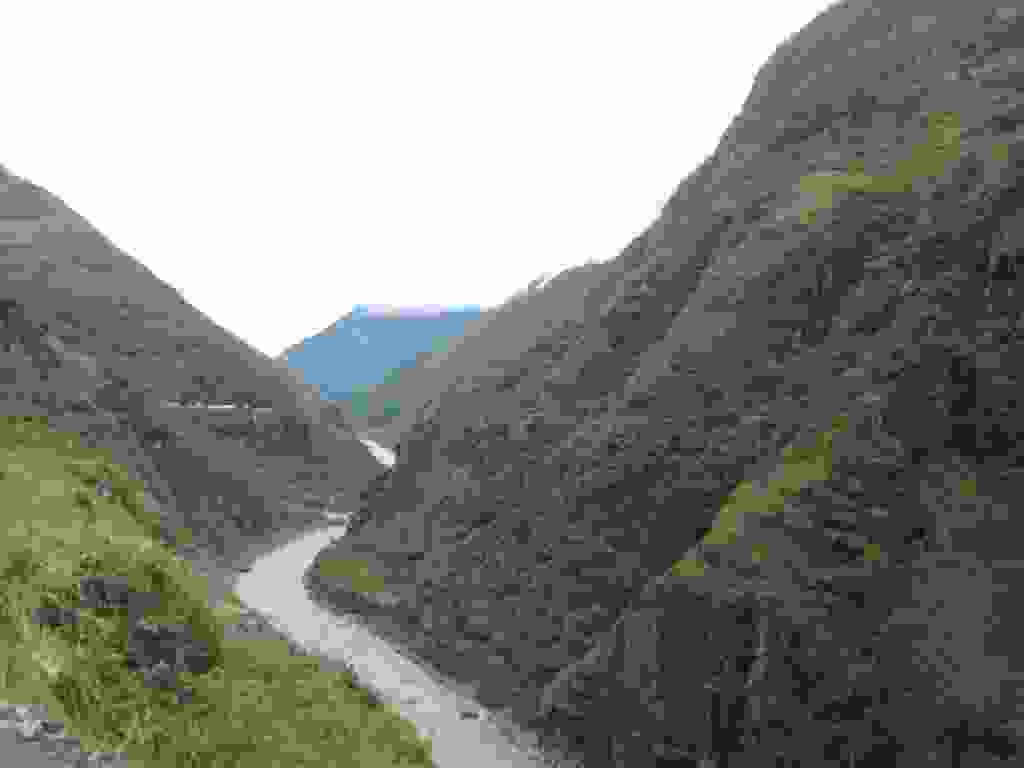
\includegraphics[height=90mm]{../wp-content/uploads/2015/06/wpid-wp-1435593846148-1024x768.jpg} } 
 \newline
 \newline
\centerline{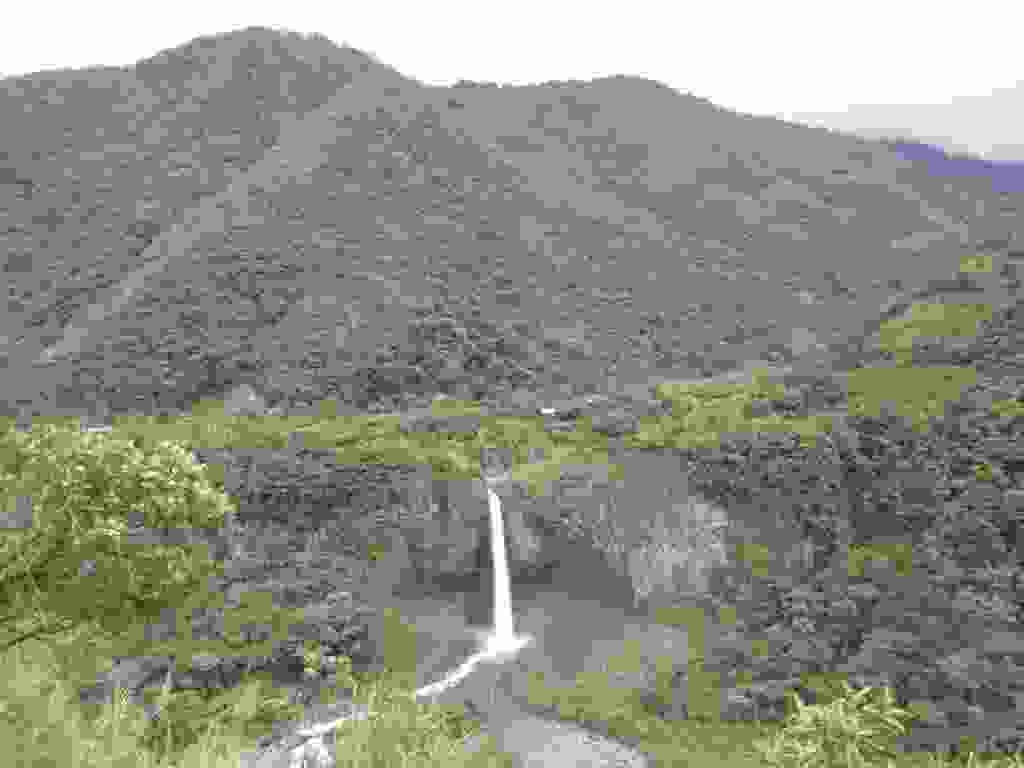
\includegraphics[height=90mm]{../wp-content/uploads/2015/06/wpid-wp-1435593861799-1024x768.jpg} } 
 \newline
 La cascade Pailon del Diablo est la plus impressionnante. \newline
 \newline
\centerline{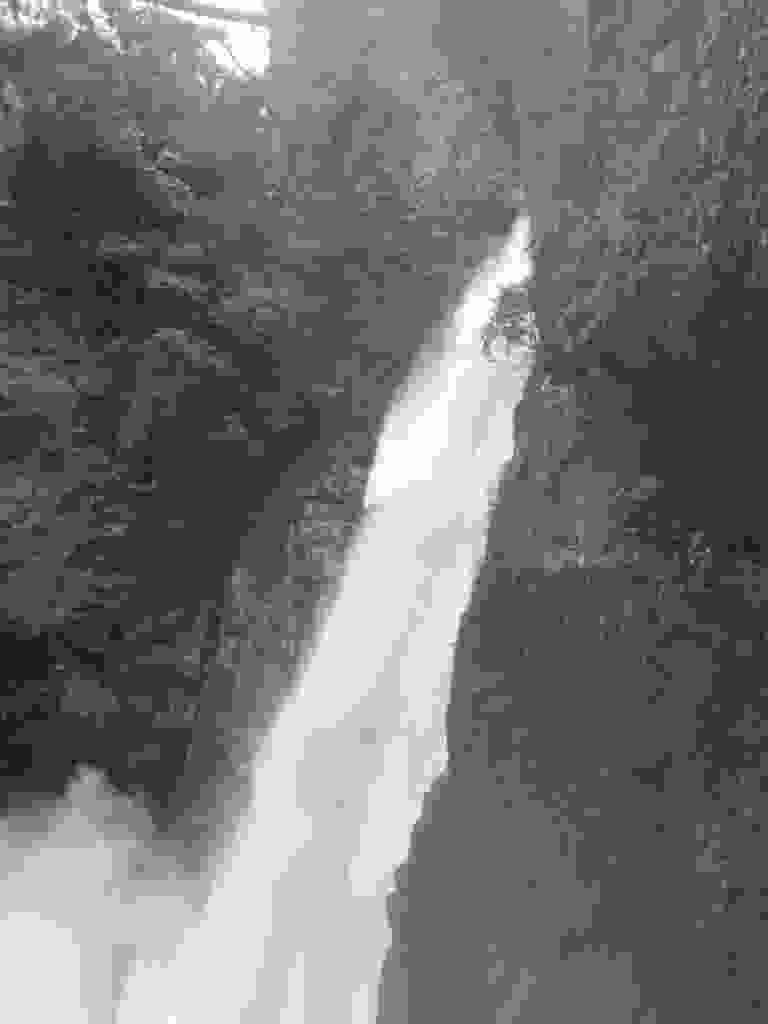
\includegraphics[height=90mm]{../wp-content/uploads/2015/06/P6224978-e1435962282463-768x1024.jpg} } 
 \newline
 \newline
\centerline{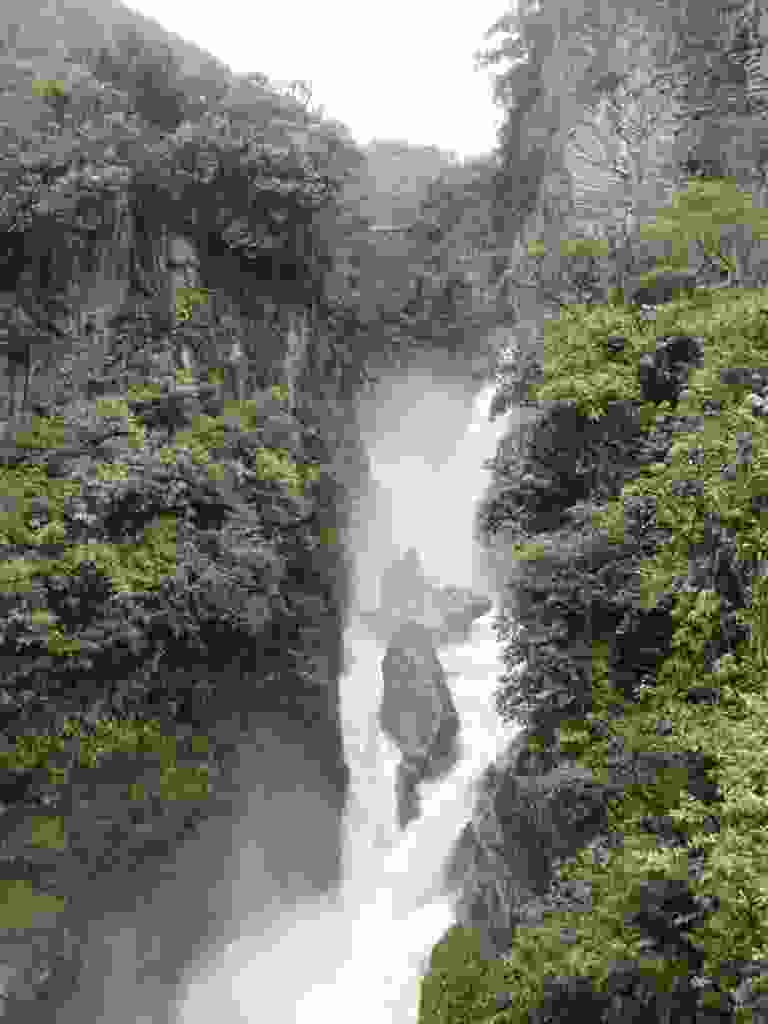
\includegraphics[height=90mm]{../wp-content/uploads/2015/06/P6224991-e1435962256922-768x1024.jpg} } 
 \newline
 J'arrive à Puyo, une petite ville située à l'entrée de la jungle. \newline
 \newline
\centerline{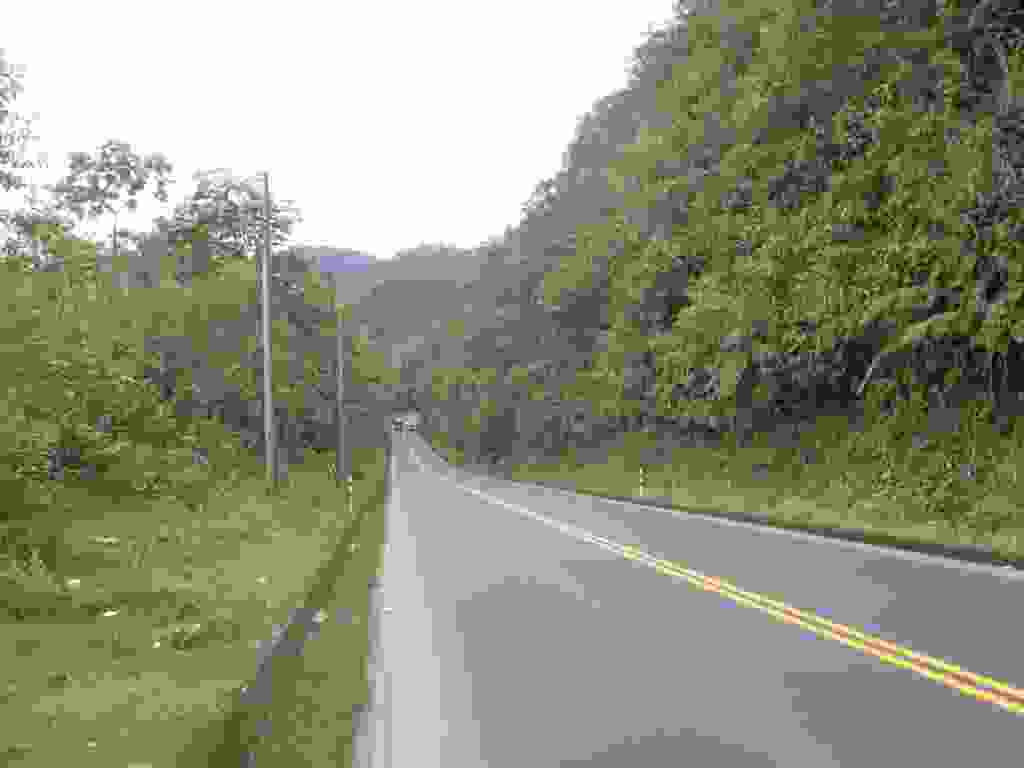
\includegraphics[height=90mm]{../wp-content/uploads/2015/06/P6224994-1024x768.jpg} } 
 \newline
 \newline
\centerline{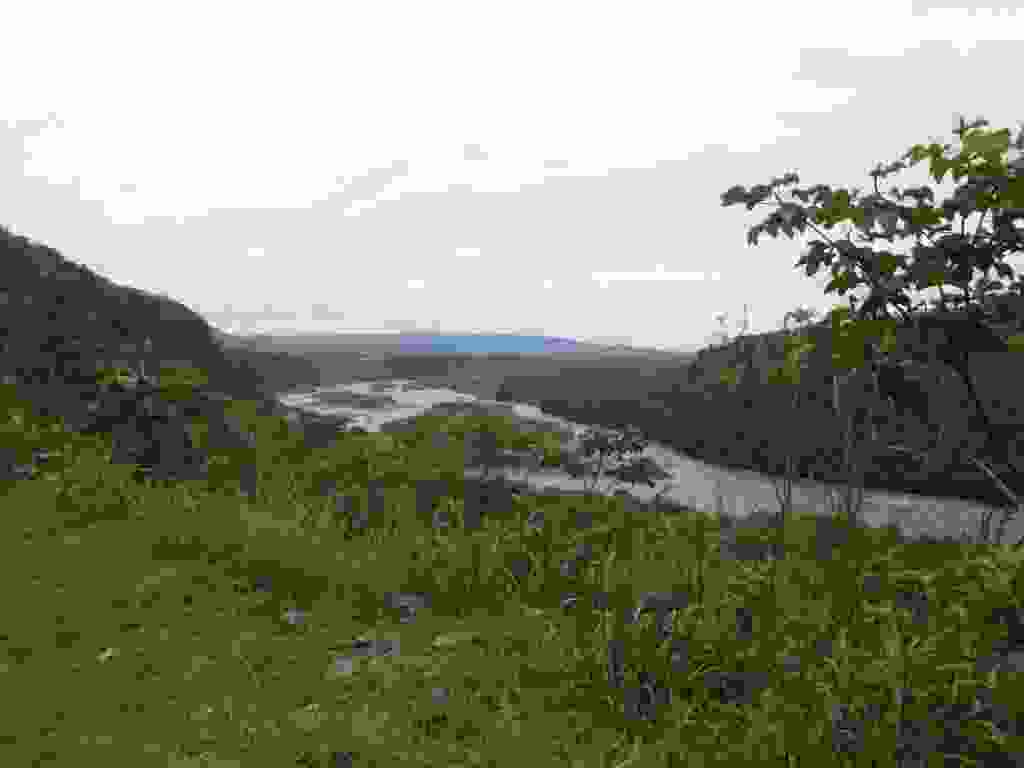
\includegraphics[height=90mm]{../wp-content/uploads/2015/06/P6224995-1024x768.jpg} } 
 \newline
 J'en profite pour passer une journée dans la jungle avec un guide local, Enrique. \newline
 La marche passe par 2 belles cascades et on peut se baigner dans la 2e. \newline
 \newline
\centerline{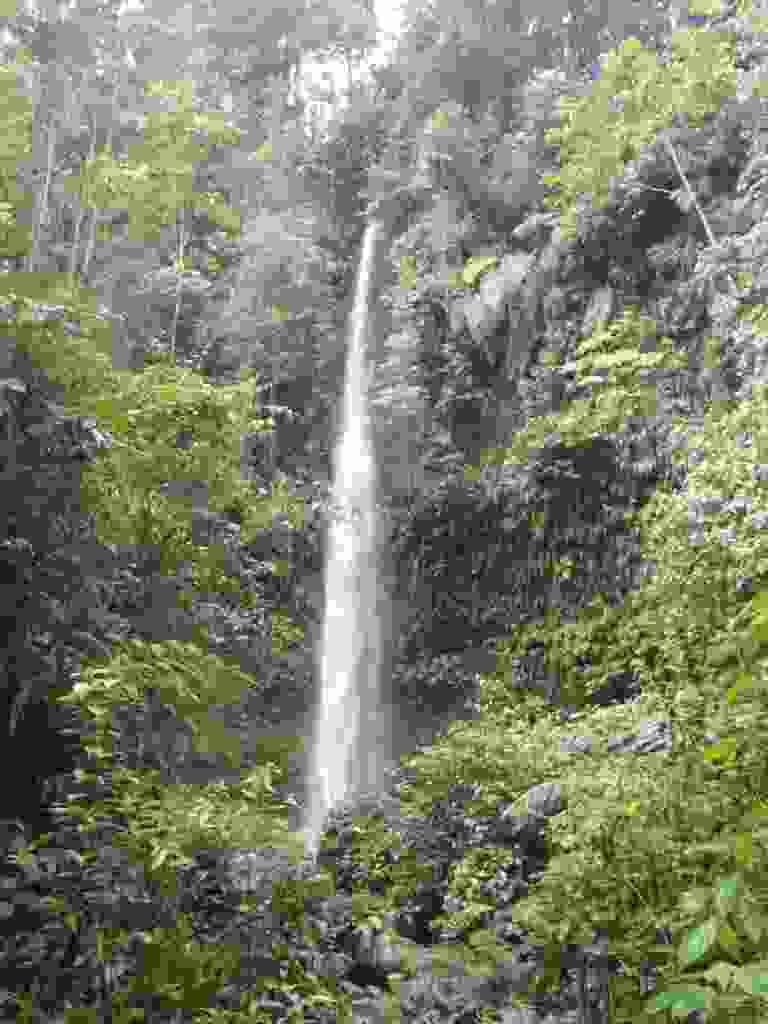
\includegraphics[height=90mm]{../wp-content/uploads/2015/06/P6235001-768x1024.jpg} } 
 \newline
 \newline
\centerline{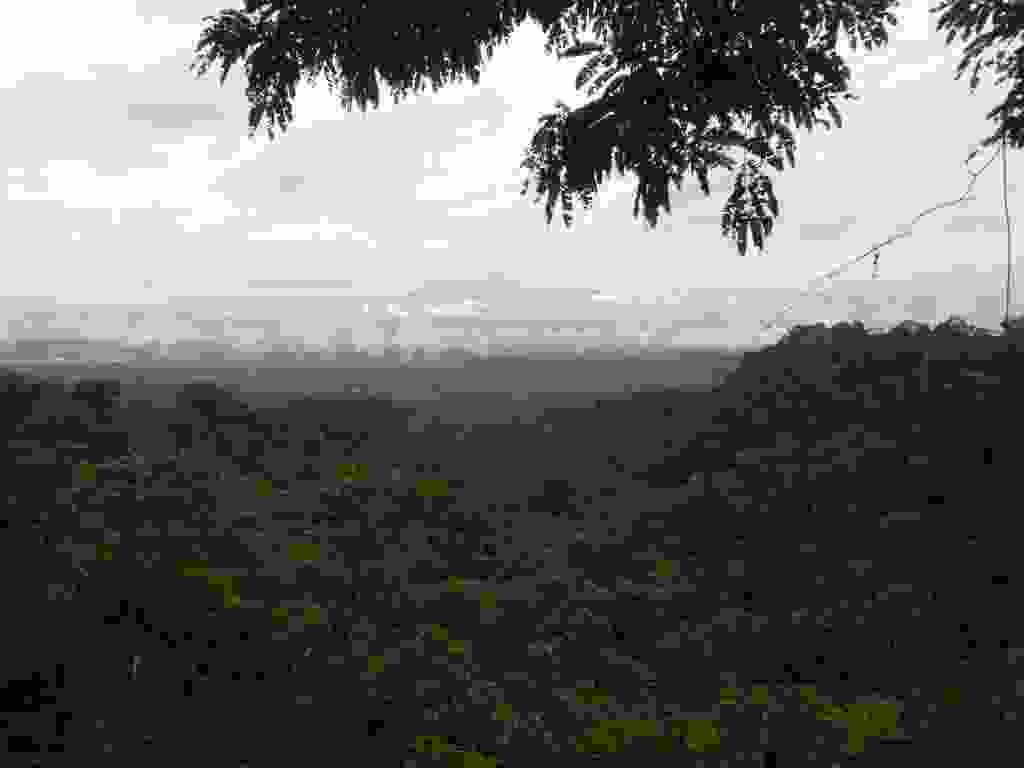
\includegraphics[height=90mm]{../wp-content/uploads/2015/06/P6235014-1024x768.jpg} } 
 \newline
 \newline
\centerline{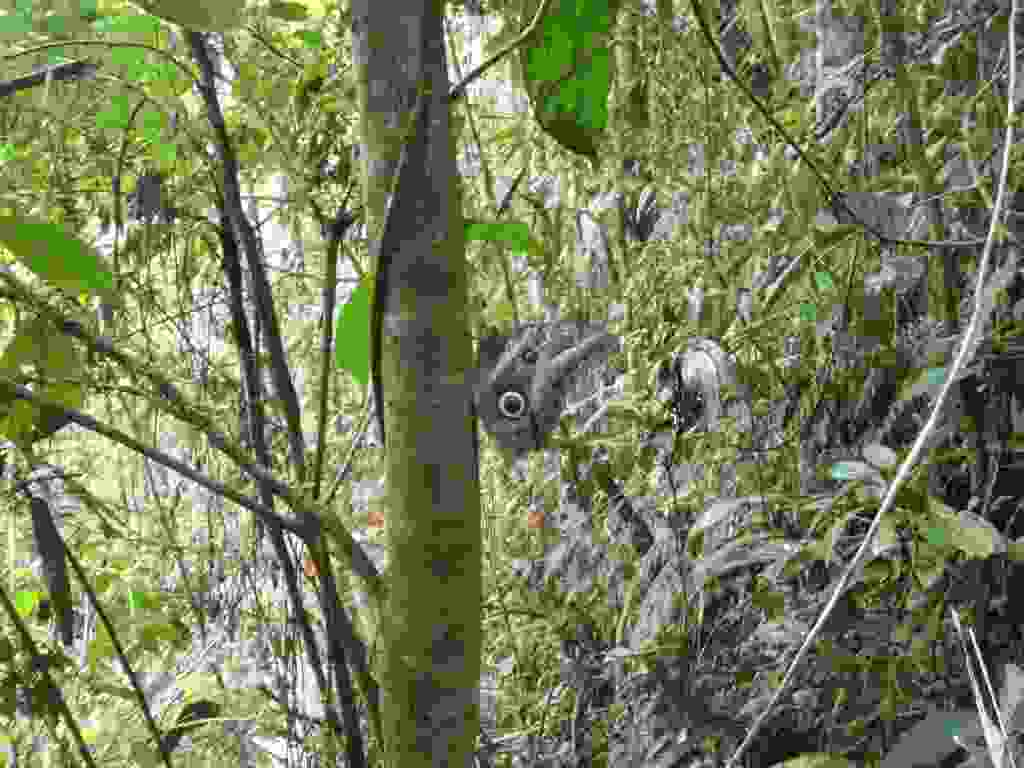
\includegraphics[height=90mm]{../wp-content/uploads/2015/06/P6235015-1024x768.jpg} } 
 \newline
 \newline
\centerline{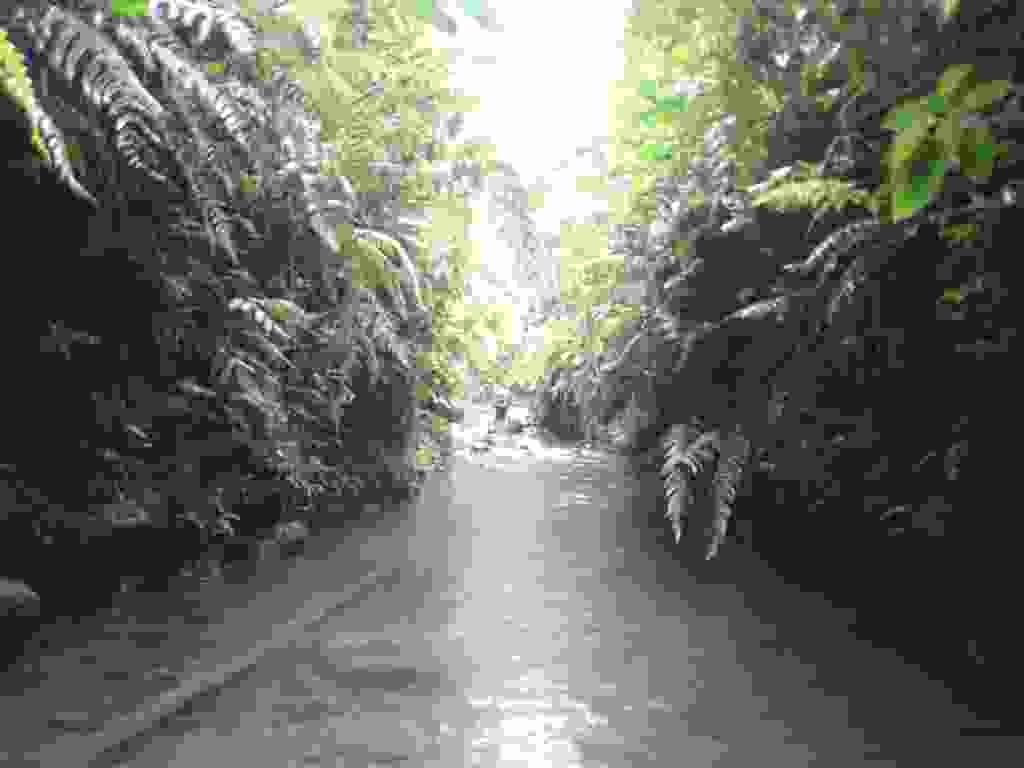
\includegraphics[height=90mm]{../wp-content/uploads/2015/06/P6235017-1024x768.jpg} } 
 \newline
 \newline
\centerline{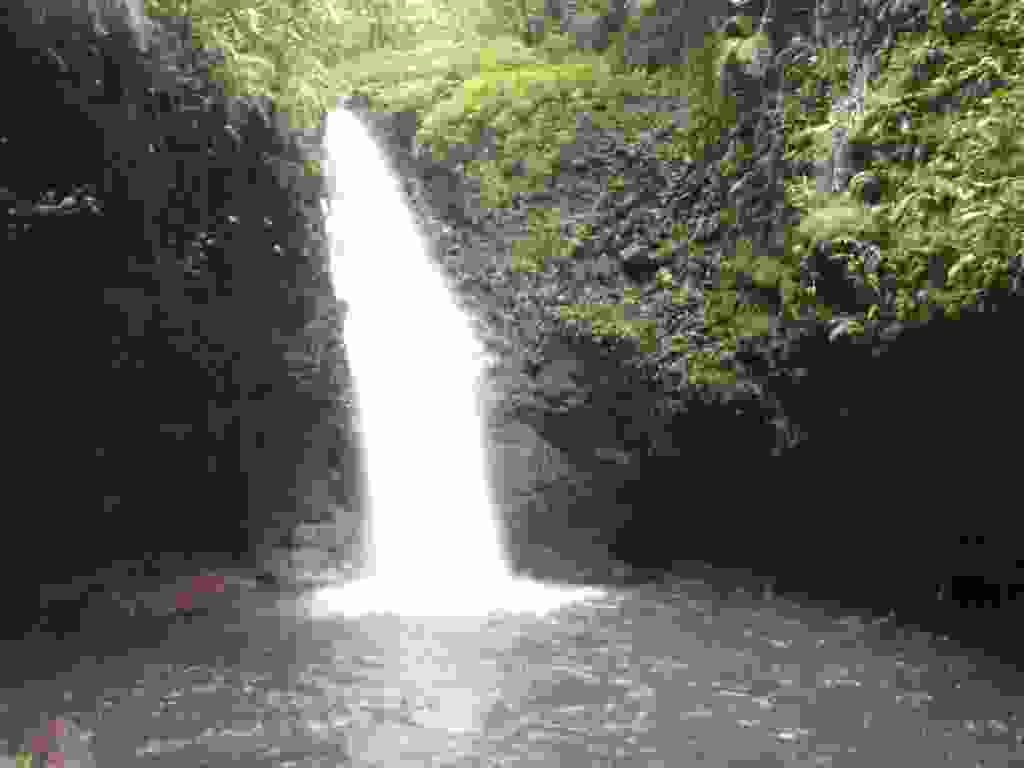
\includegraphics[height=90mm]{../wp-content/uploads/2015/06/P6235020-1024x768.jpg} } 
 \newline
 Des dizaines d´oiseaux qui s´envolent quand on arrive. \newline
 \newline
\centerline{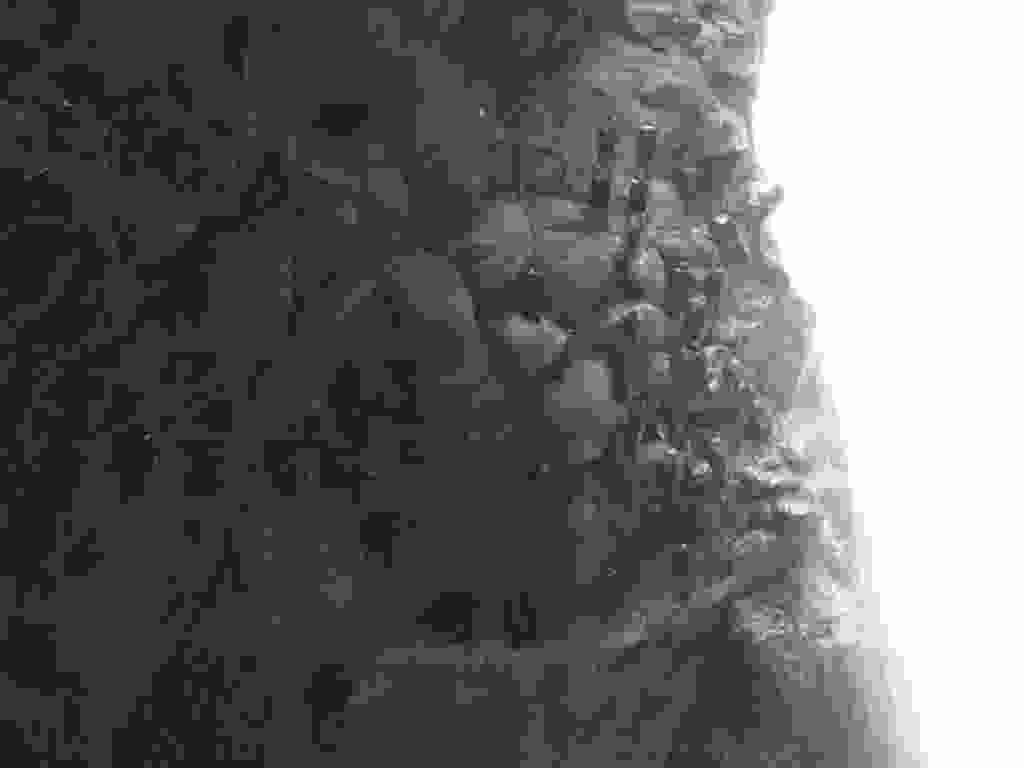
\includegraphics[height=90mm]{../wp-content/uploads/2015/06/P6235022-1024x768.jpg} } 
 \newline
 Passage par une communauté indigène. \newline
 \newline
\centerline{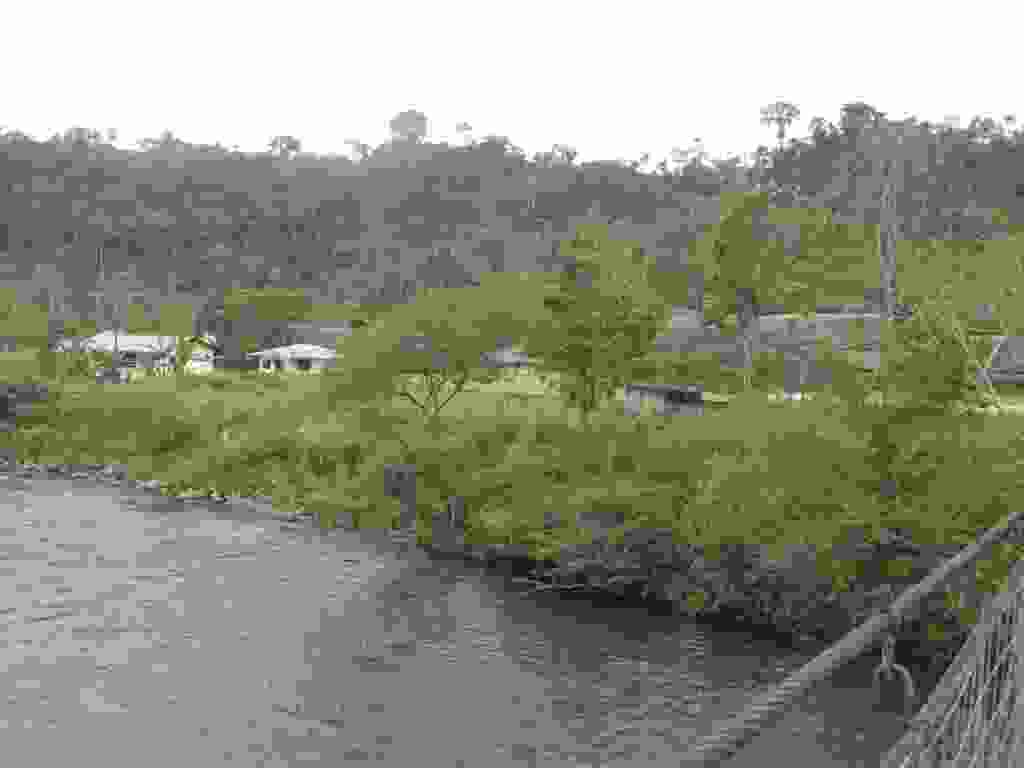
\includegraphics[height=90mm]{../wp-content/uploads/2015/06/P6235035-1024x768.jpg} } 
 \newline
 Le temps de se faire peindre le visage avant une balade en barque sur la rivière. \newline
 \newline
\centerline{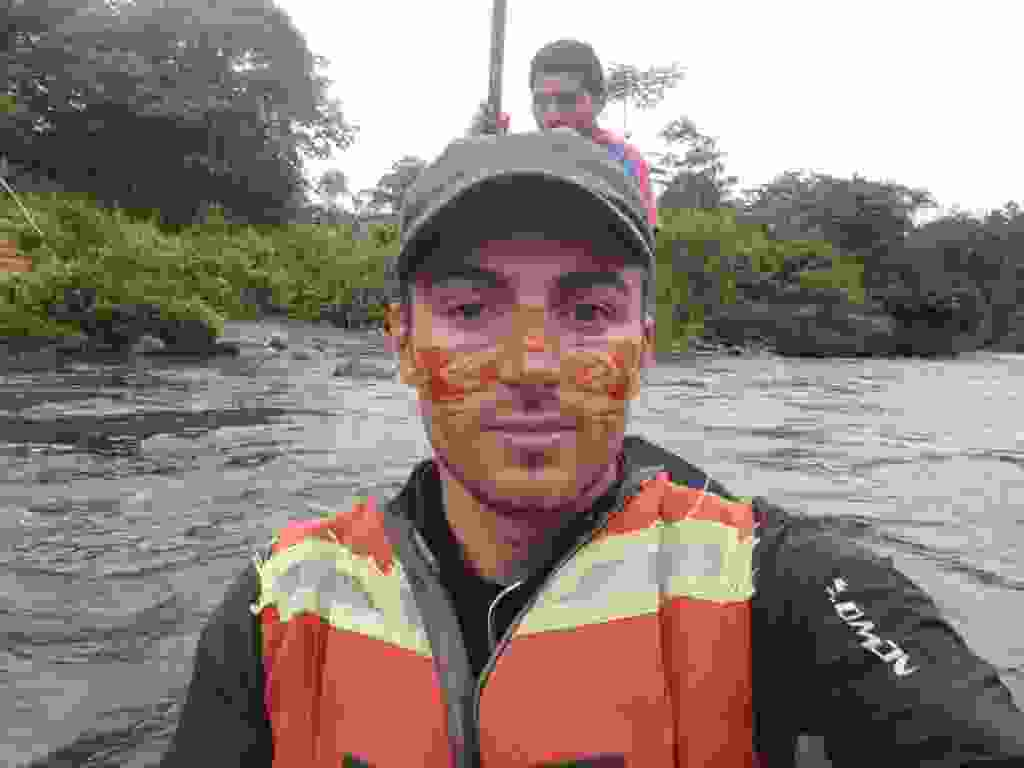
\includegraphics[height=90mm]{../wp-content/uploads/2015/06/P6235046-1024x768.jpg} } 
 \newline
 \newline
\centerline{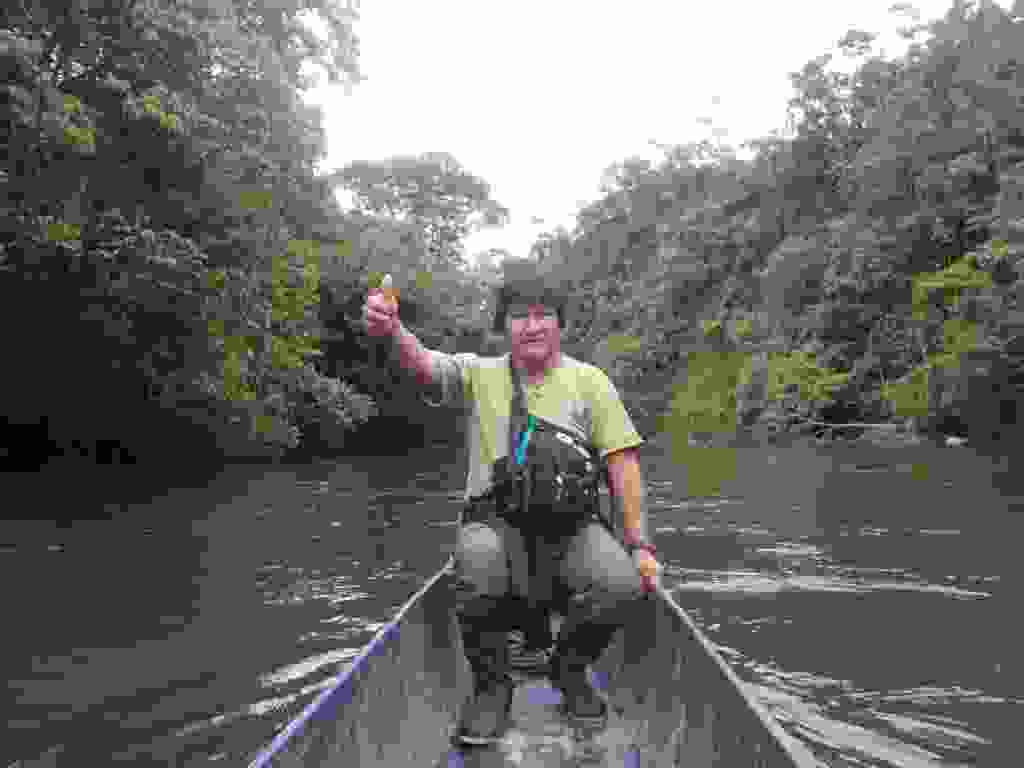
\includegraphics[height=90mm]{../wp-content/uploads/2015/06/P6235051-1024x768.jpg} } 
 \newline
 Mirador sur la jungle. \newline
 \newline
\centerline{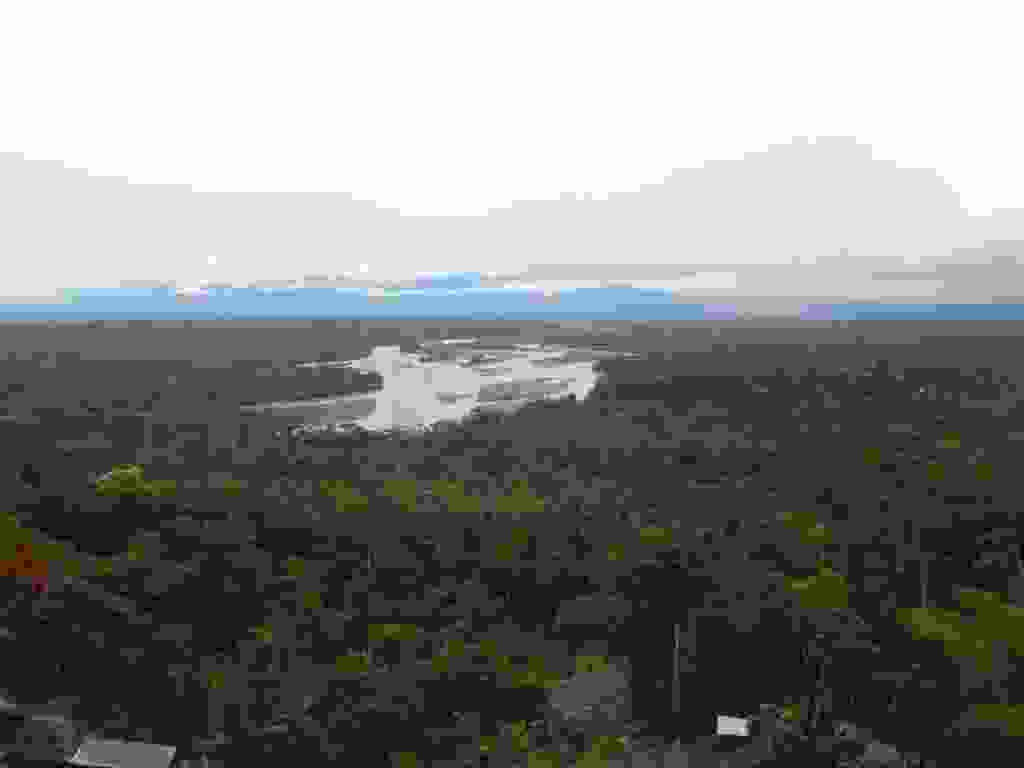
\includegraphics[height=90mm]{../wp-content/uploads/2015/06/P6235060-1024x768.jpg} } 
 \newline
 Des ananas sur le chemin. \newline
 \newline
\centerline{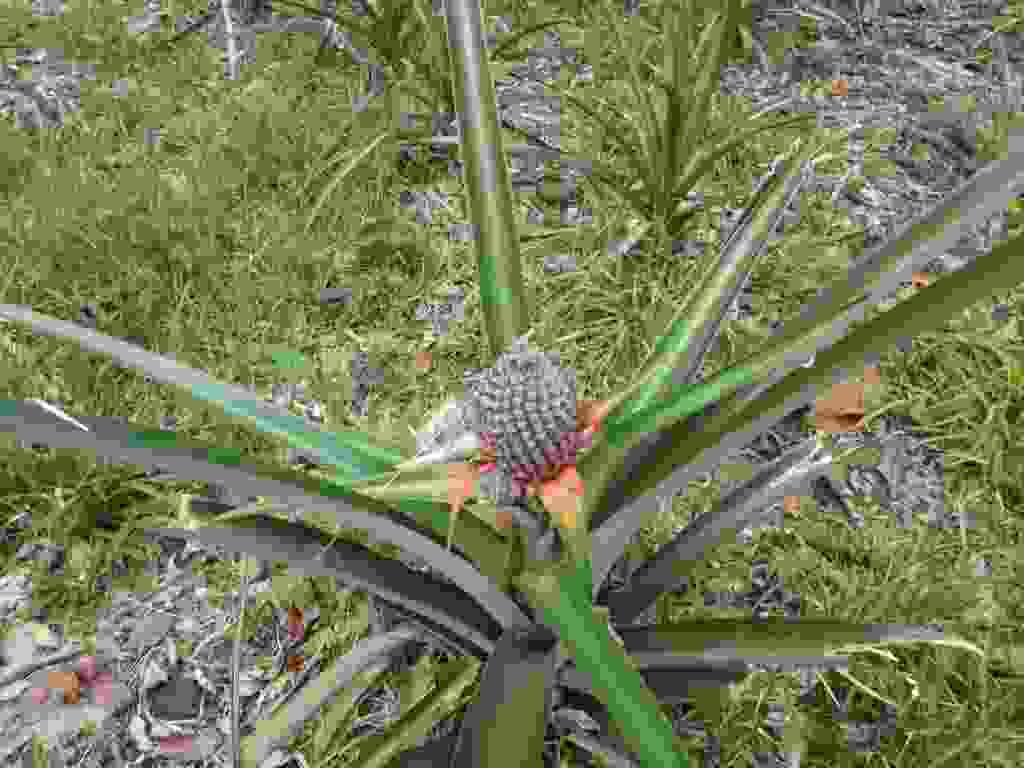
\includegraphics[height=90mm]{../wp-content/uploads/2015/06/P6235063-1024x768.jpg} } 
 \newline
 Le lac aux crocodiles. \newline
 \newline
\centerline{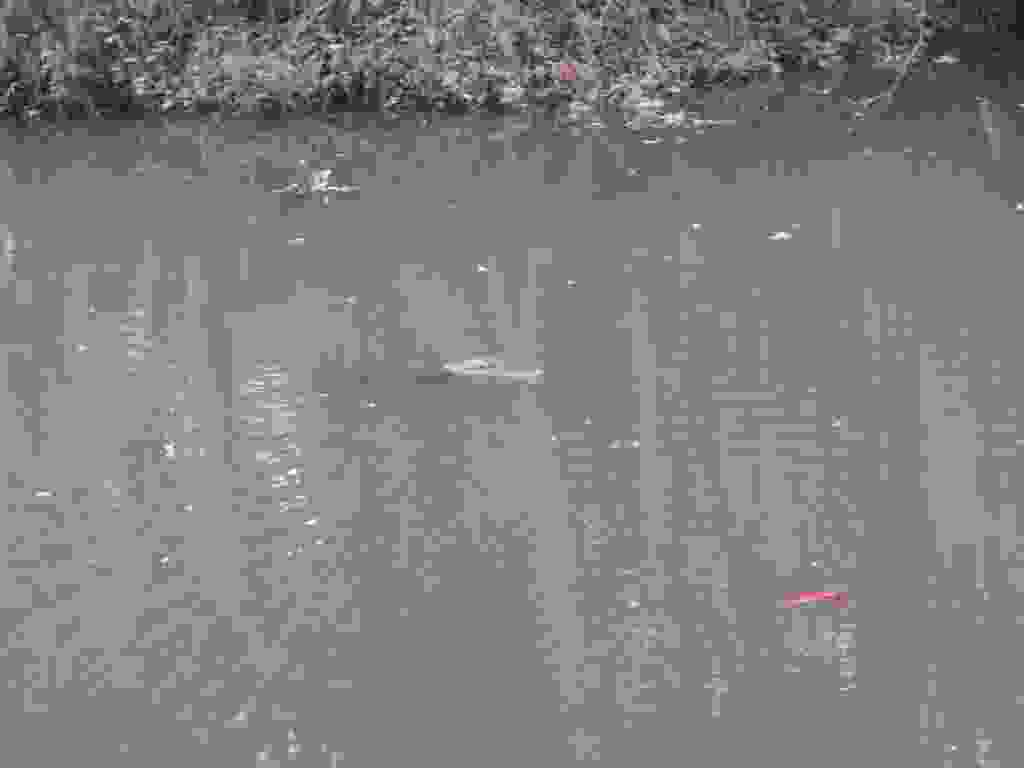
\includegraphics[height=90mm]{../wp-content/uploads/2015/06/P6235070-1024x768.jpg} } 
 \newline
 La journée se termine dans la propriété familiale de Enrique ou j´assiste à la fabrication de meubles artisanaux. \newline
 \newline
\centerline{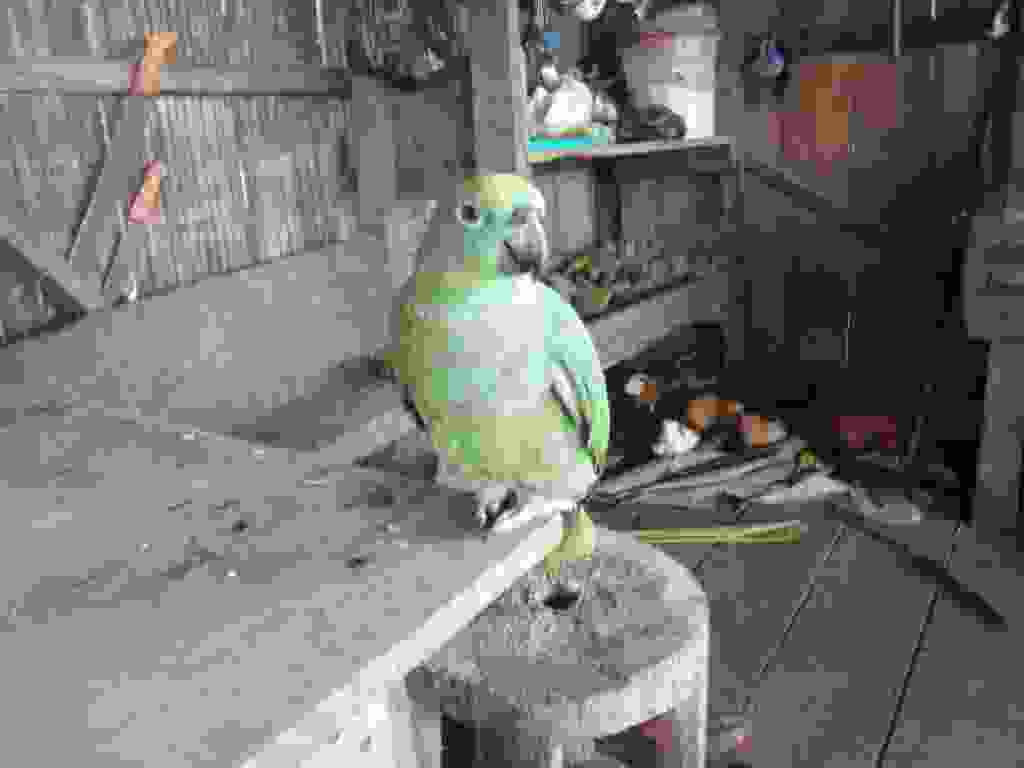
\includegraphics[height=90mm]{../wp-content/uploads/2015/06/P6235074-1024x768.jpg} } 
 \newline
 \newline
\centerline{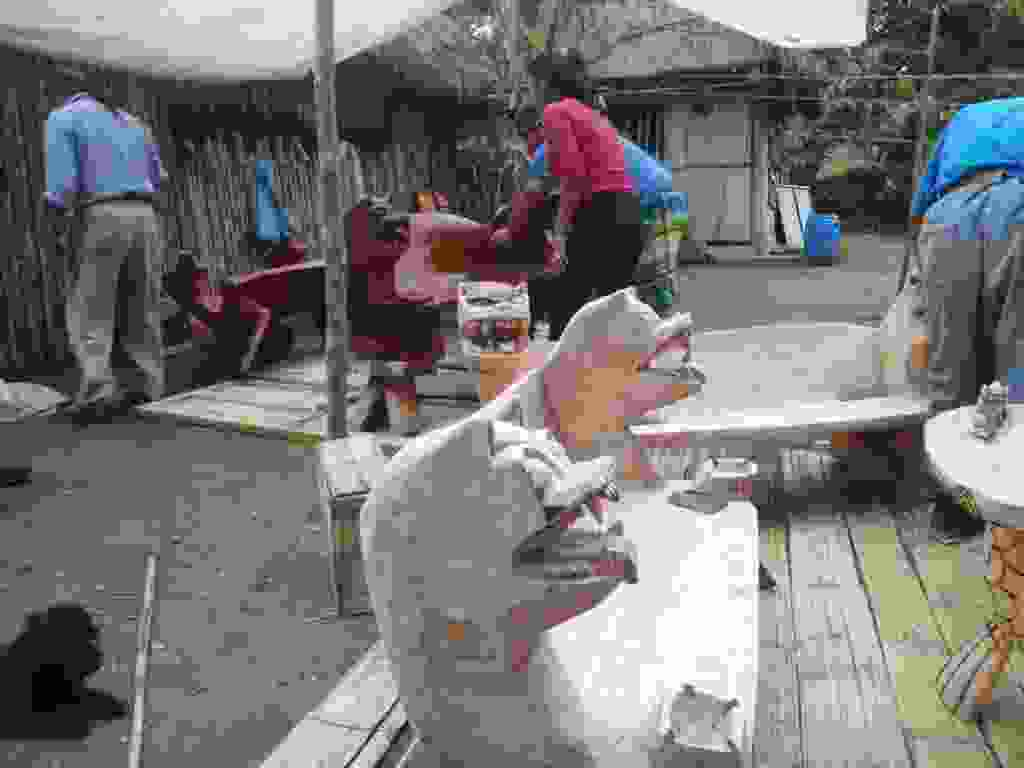
\includegraphics[height=90mm]{../wp-content/uploads/2015/06/P6235077-1024x768.jpg} } 
 \newline
 Je remonte ensuite sur la route vers Quito. \newline
 \newline
\centerline{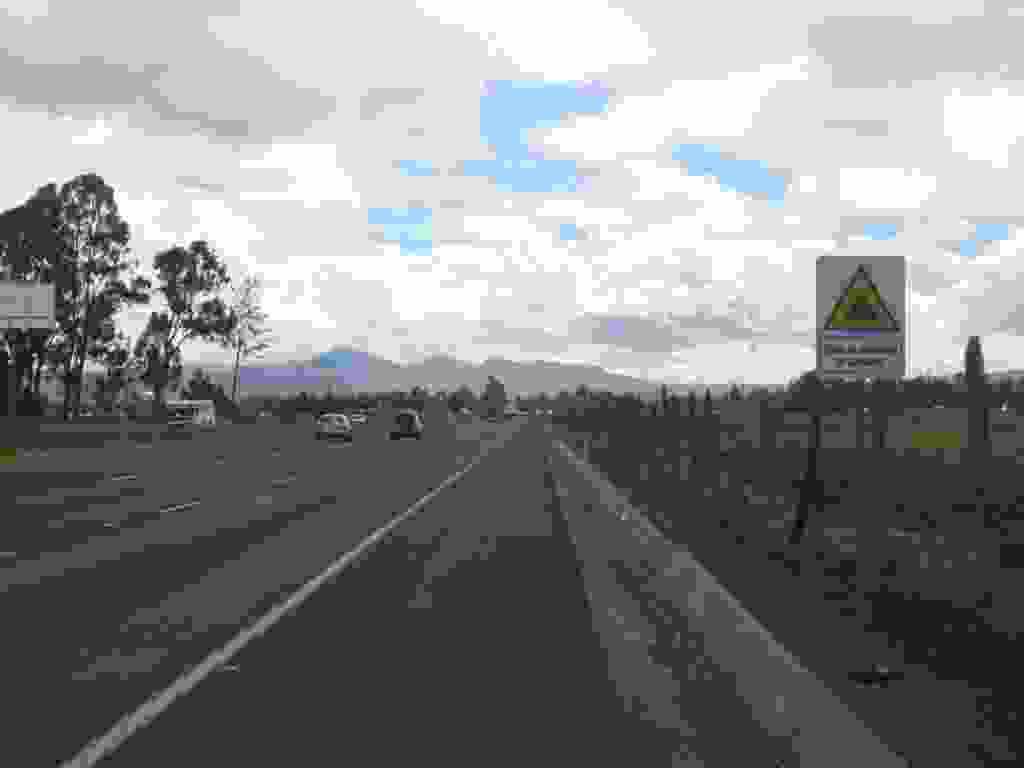
\includegraphics[height=90mm]{../wp-content/uploads/2015/06/P6255087-1024x768.jpg} } 
 \newline
 Je fais étape a Latacunga, pour une sympathique soirée chez Javier et sa famille. \newline
 \newline
\centerline{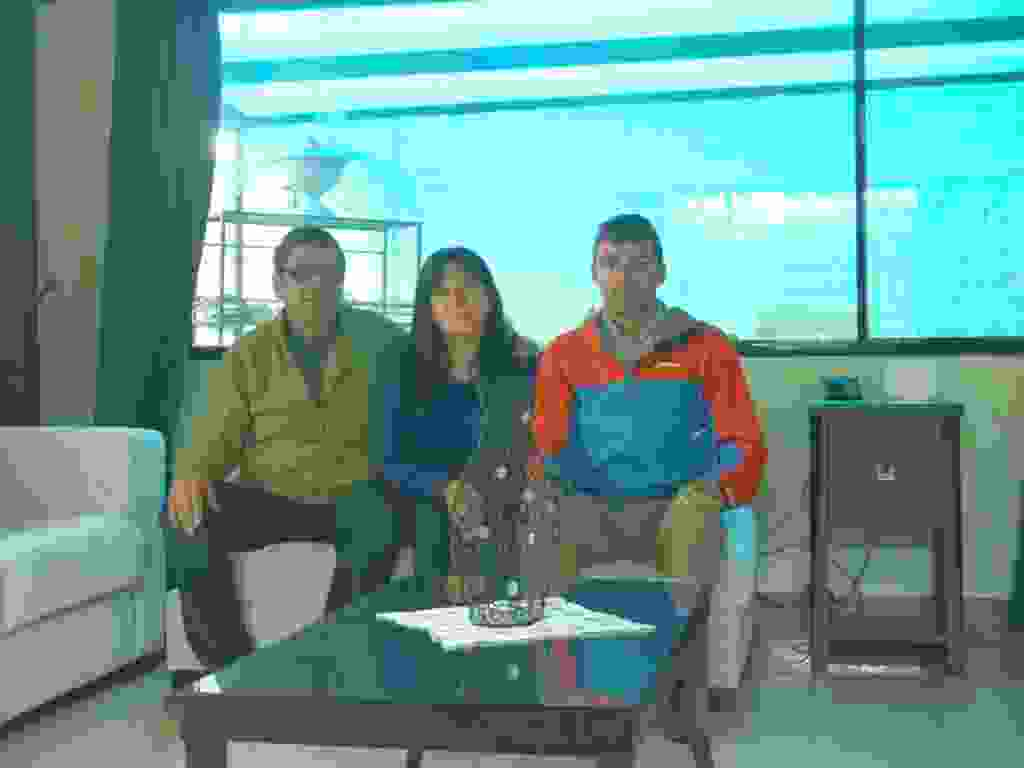
\includegraphics[height=90mm]{../wp-content/uploads/2015/06/P6255084-1024x768.jpg} } 
 \newline
 La route me mène dans le parc national Cotopaxi. \newline
 \newline
\centerline{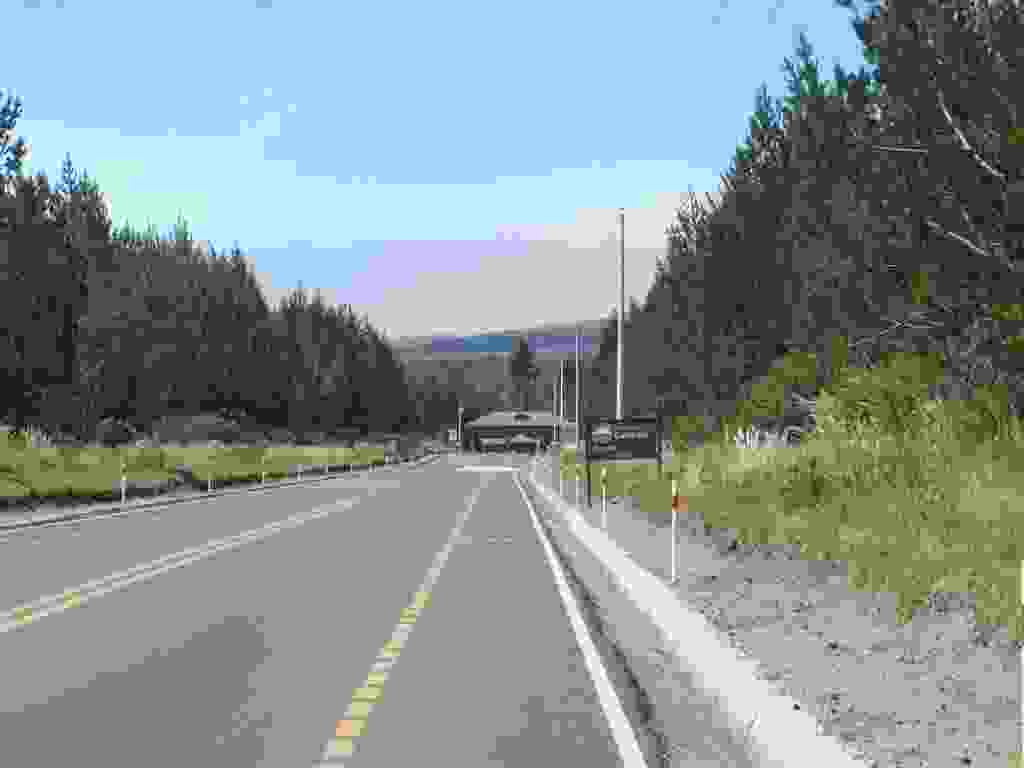
\includegraphics[height=90mm]{../wp-content/uploads/2015/06/P6255095-1024x768.jpg} } 
 \newline
 Le Cotopaxi est un volcan actif qui culmine à 5800m. \newline
 \newline
\centerline{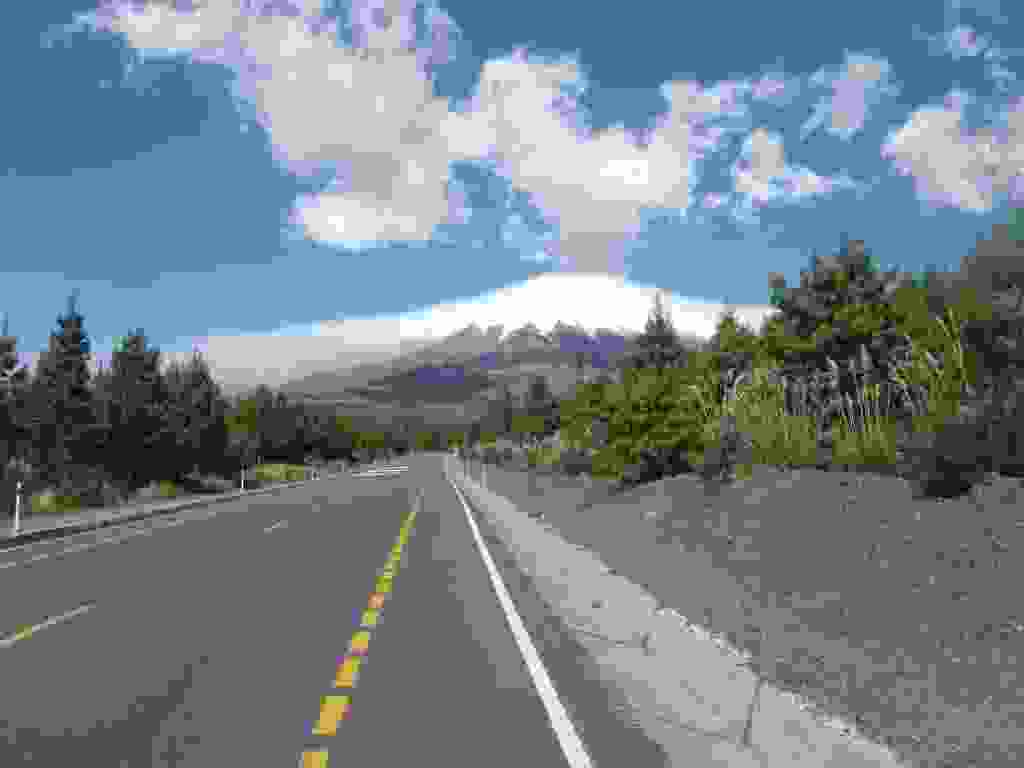
\includegraphics[height=90mm]{../wp-content/uploads/2015/06/P6255097-1024x768.jpg} } 
 \newline
 \newline
\centerline{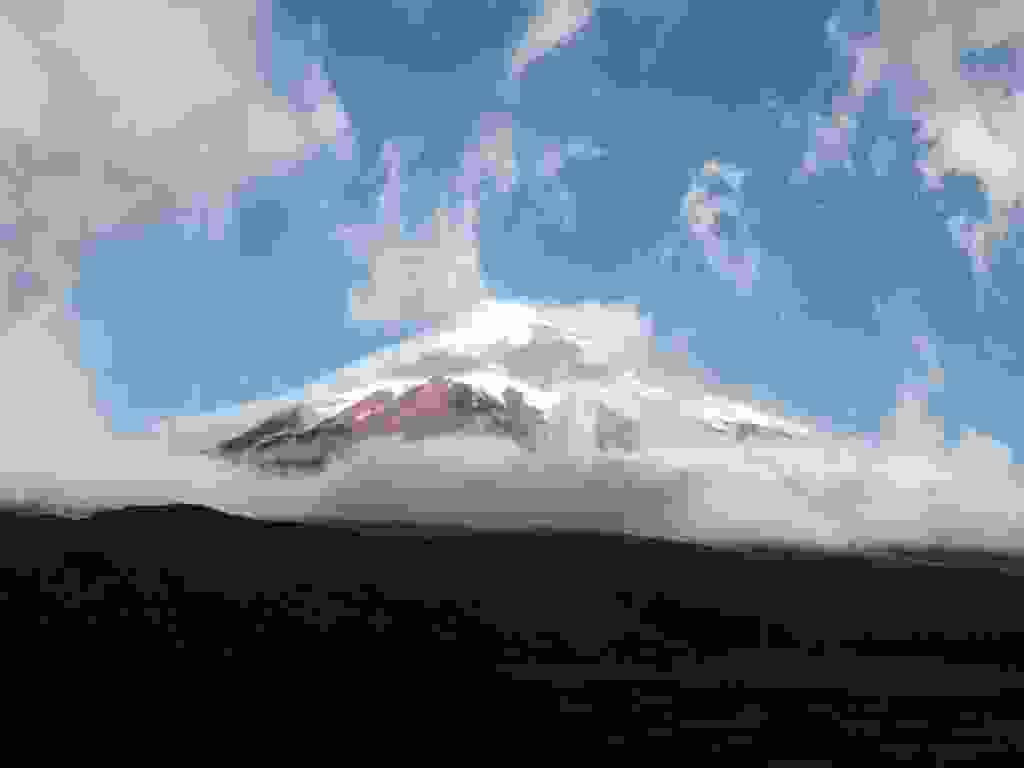
\includegraphics[height=90mm]{../wp-content/uploads/2015/06/P6265107-1024x768.jpg} } 
 \newline
 Je passe la nuit dans le camping du parc, pas d´autres campeurs ce jour lá. \newline
 \newline
\centerline{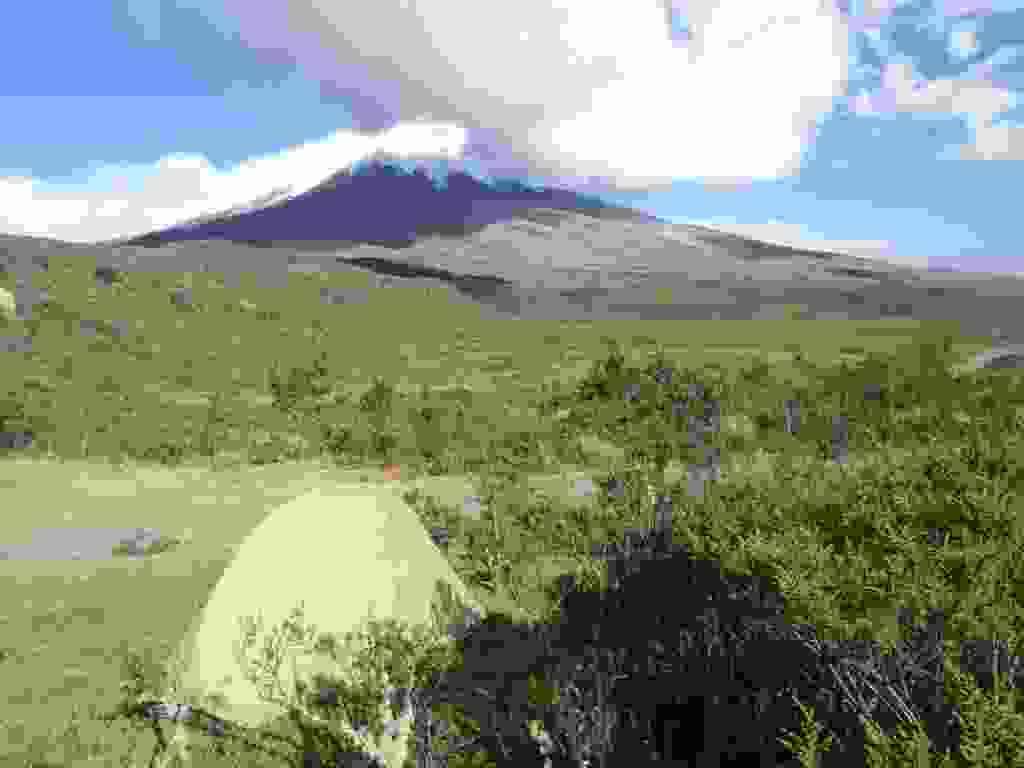
\includegraphics[height=90mm]{../wp-content/uploads/2015/06/P6255104-1024x768.jpg} } 
 \newline
 Le lendemain je monte à la Laguna Limpiopungo à 3800m. \newline
 \newline
\centerline{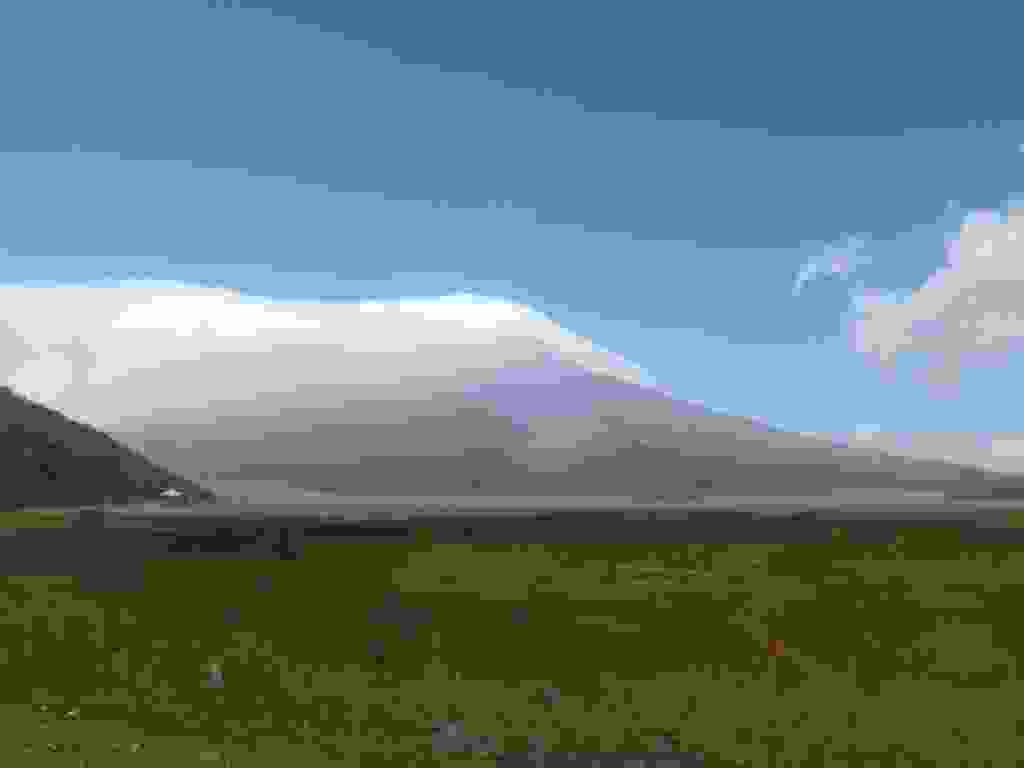
\includegraphics[height=90mm]{../wp-content/uploads/2015/06/P6265111-1024x768.jpg} } 
 \newline
 Là haut le vent est très fort et m'empêche de continuer plus loin. \newline
 Je reviens donc sur la route principale vers Quito. \newline
 \newline
\centerline{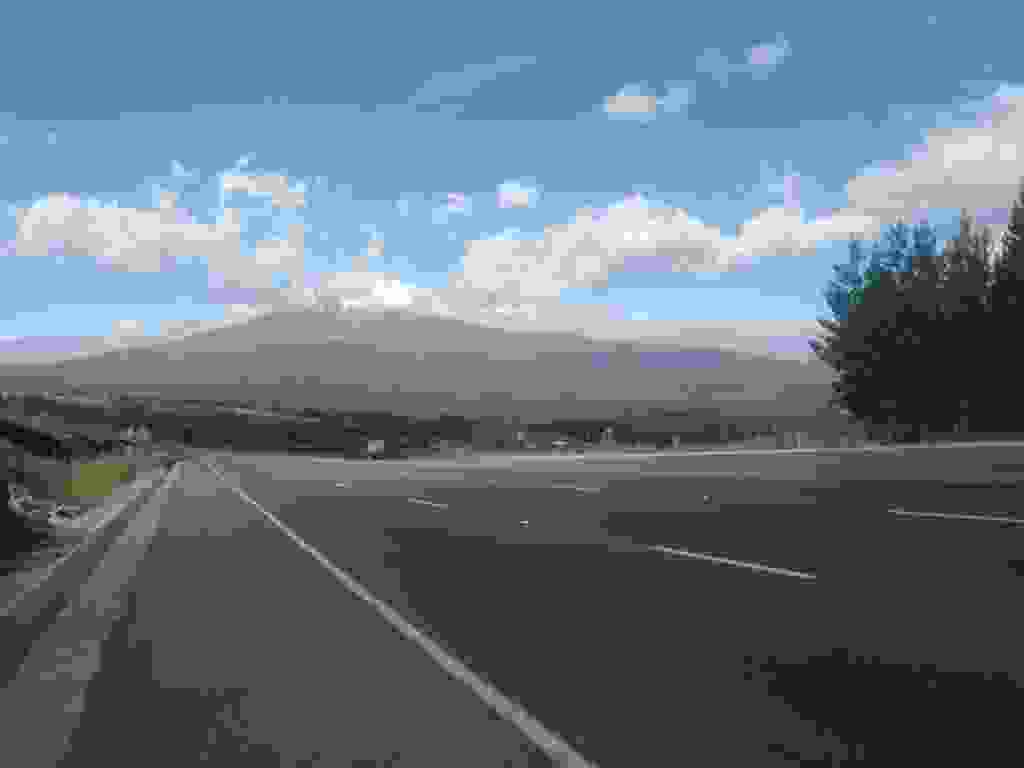
\includegraphics[height=90mm]{../wp-content/uploads/2015/06/P6265115-1024x768.jpg} } 
 \newline
 J´arrive à Sangolqui, ville de la banlieue ou je suis hébergé par Pablo et sa famille : un accueil excellent ! \newline
 \newline
\centerline{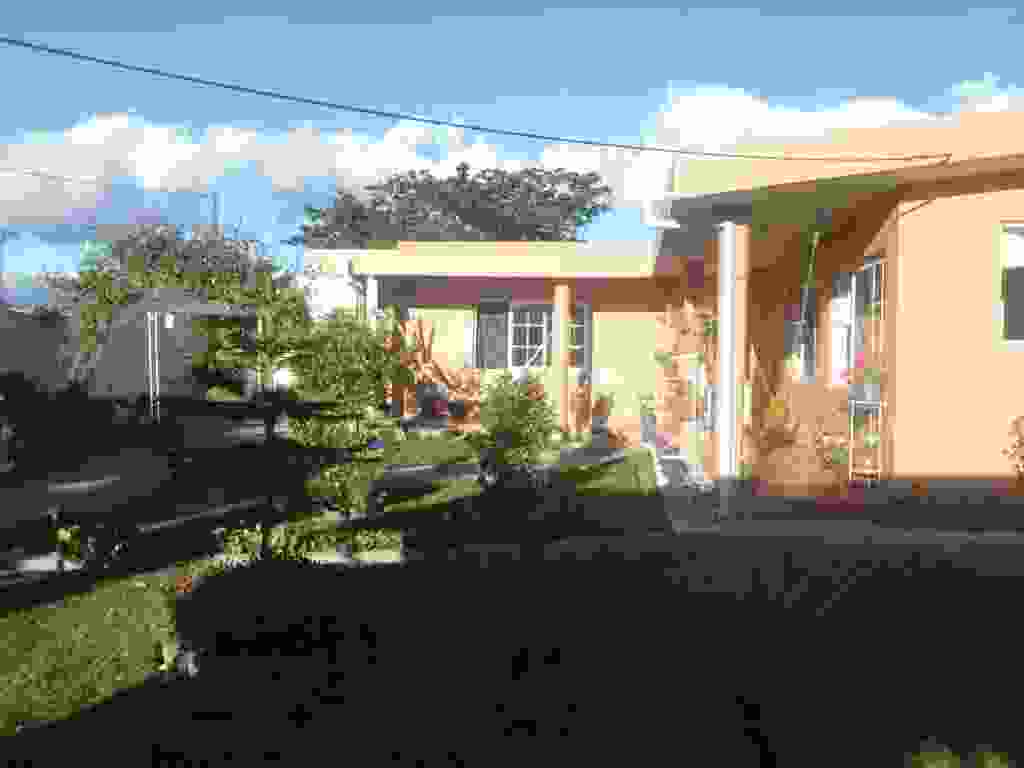
\includegraphics[height=90mm]{../wp-content/uploads/2015/06/P6275118-1024x768.jpg} } 
 \newline
 \newline
\centerline{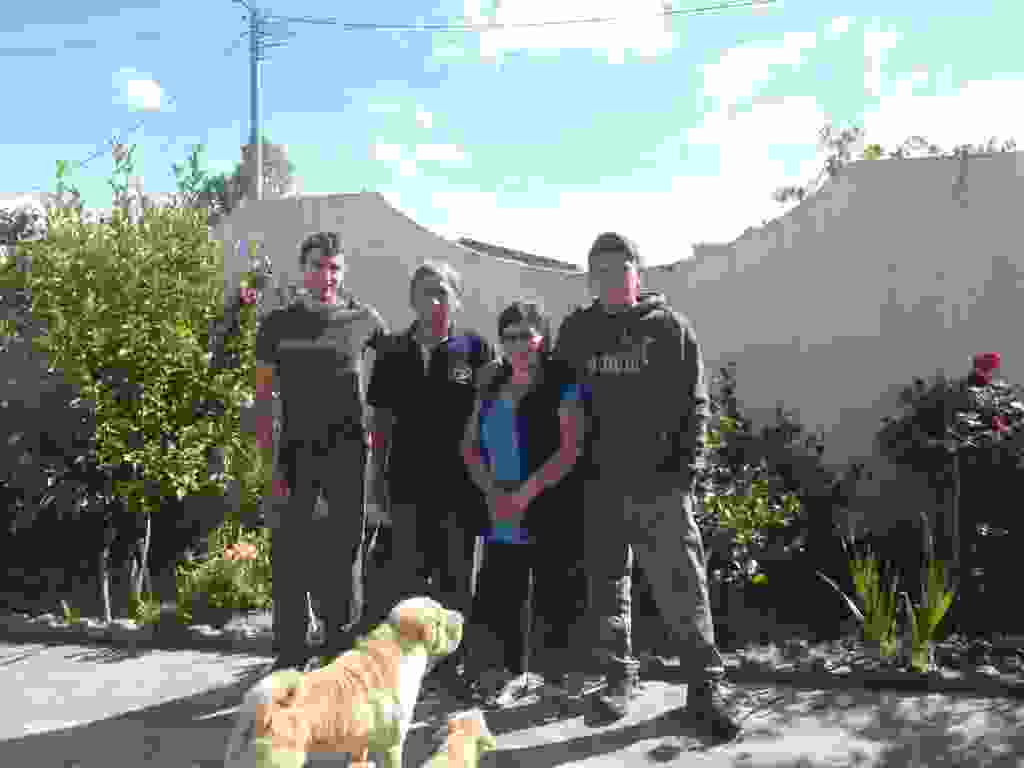
\includegraphics[height=90mm]{../wp-content/uploads/2015/06/P6295144-1024x768.jpg} } 
 \newline
 Balade sur une petite montagne proche avec Pablo et un cousin. \newline
 \newline
\centerline{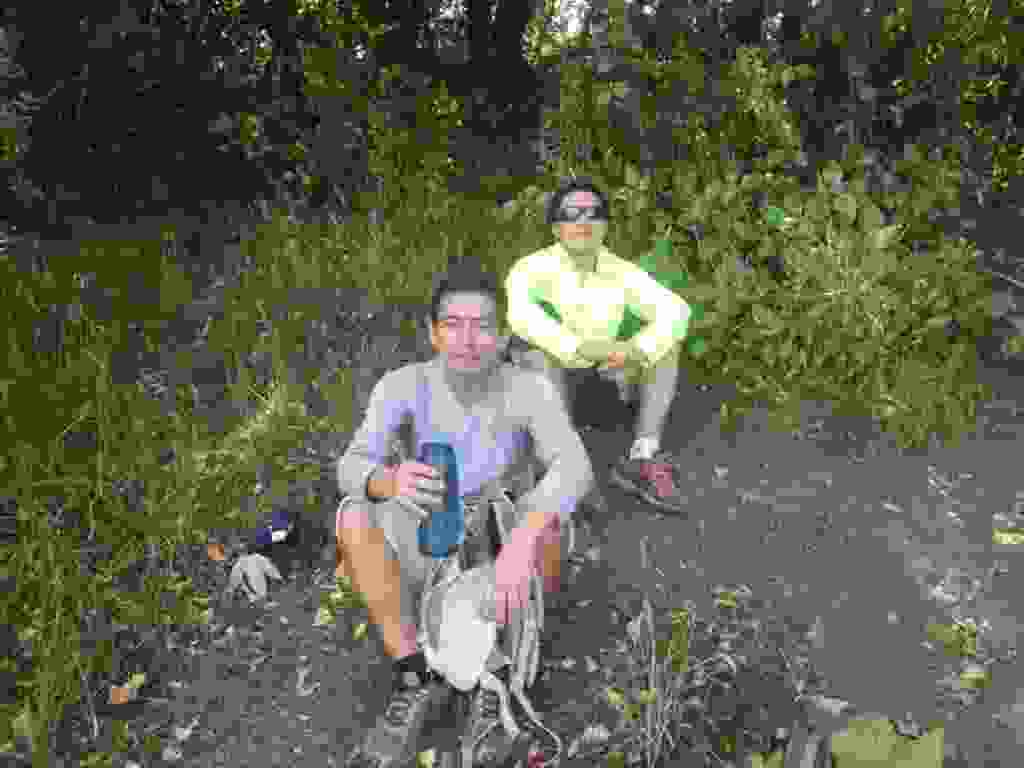
\includegraphics[height=90mm]{../wp-content/uploads/2015/06/P6285136-1024x768.jpg} } 
 \newline
 \newline
\centerline{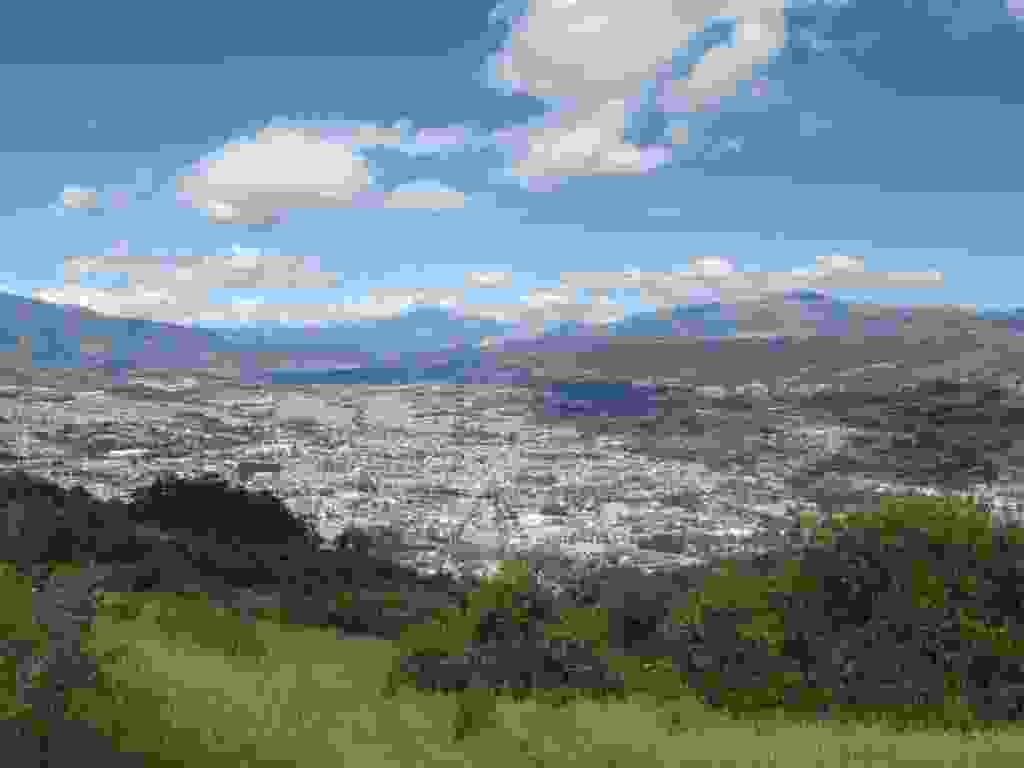
\includegraphics[height=90mm]{../wp-content/uploads/2015/06/P6285132-1024x768.jpg} } 
 \newline
 \newline
\centerline{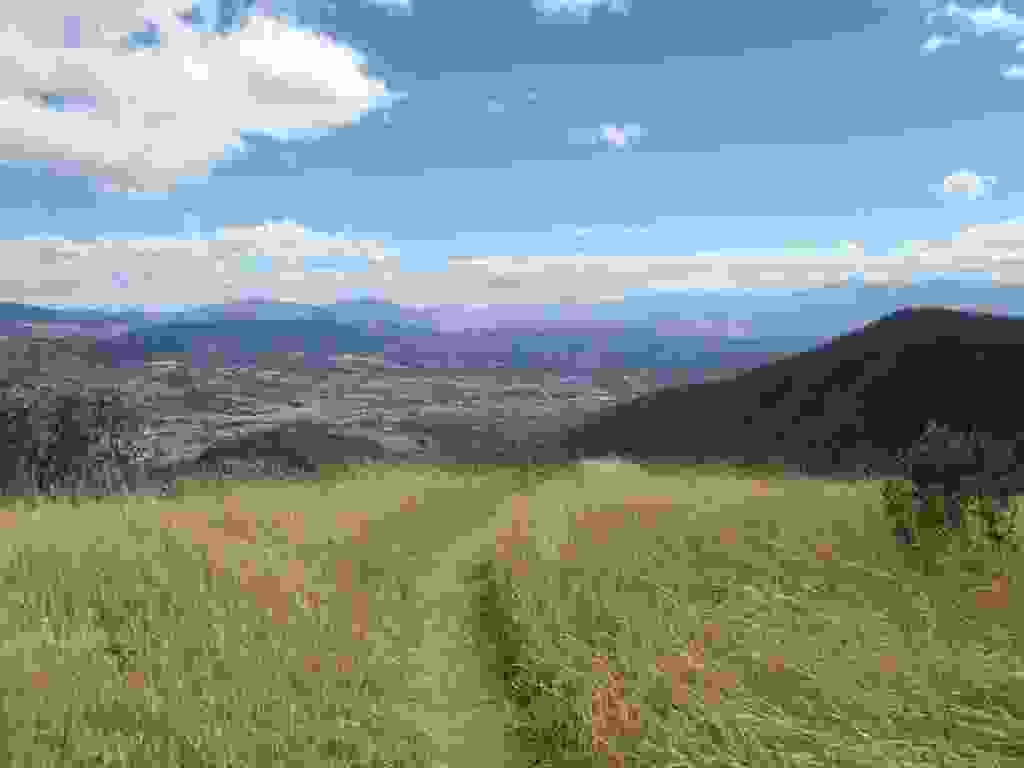
\includegraphics[height=90mm]{../wp-content/uploads/2015/06/P6285140-1024x768.jpg} } 
 \newline
 Je visite le centre historique de Quito. \newline
 \newline
\centerline{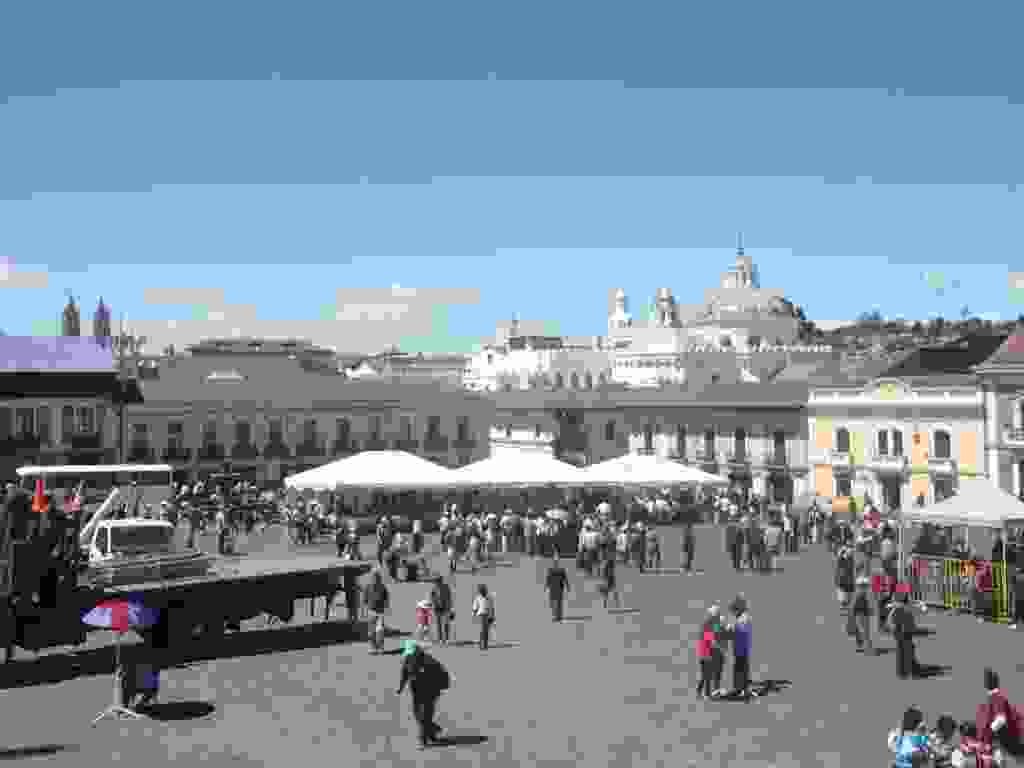
\includegraphics[height=90mm]{../wp-content/uploads/2015/06/P6275127-1024x768.jpg} } 
 \newline
 \newline
\centerline{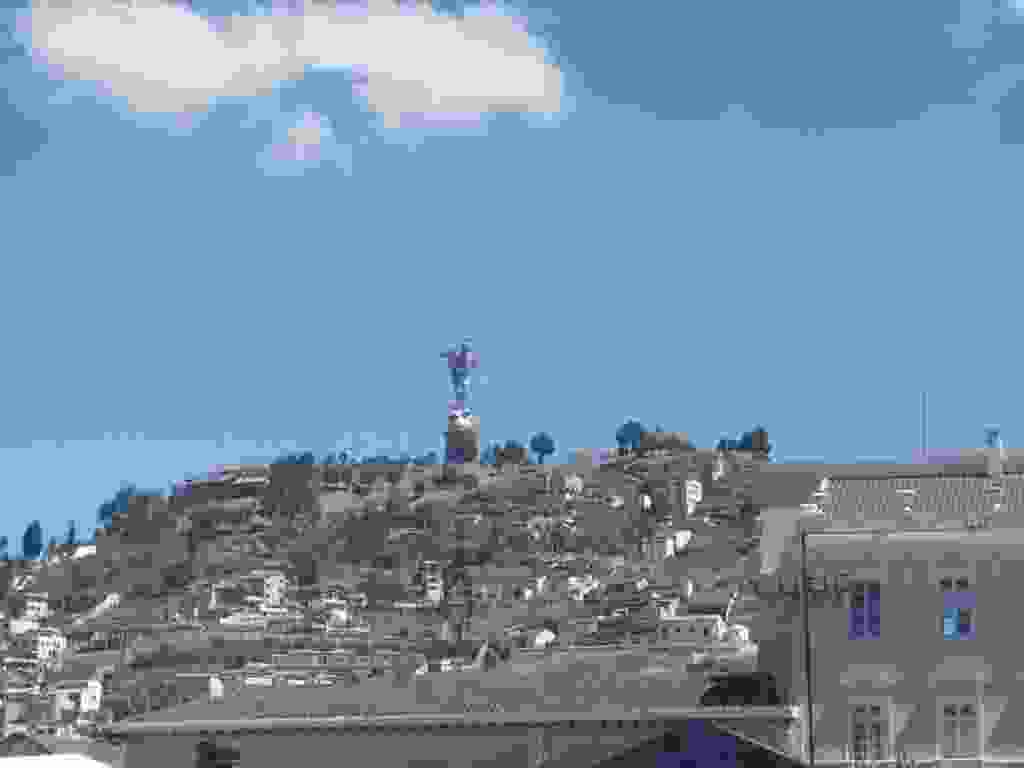
\includegraphics[height=90mm]{../wp-content/uploads/2015/06/P6275128-1024x768.jpg} } 
 \newline
 \newline
\centerline{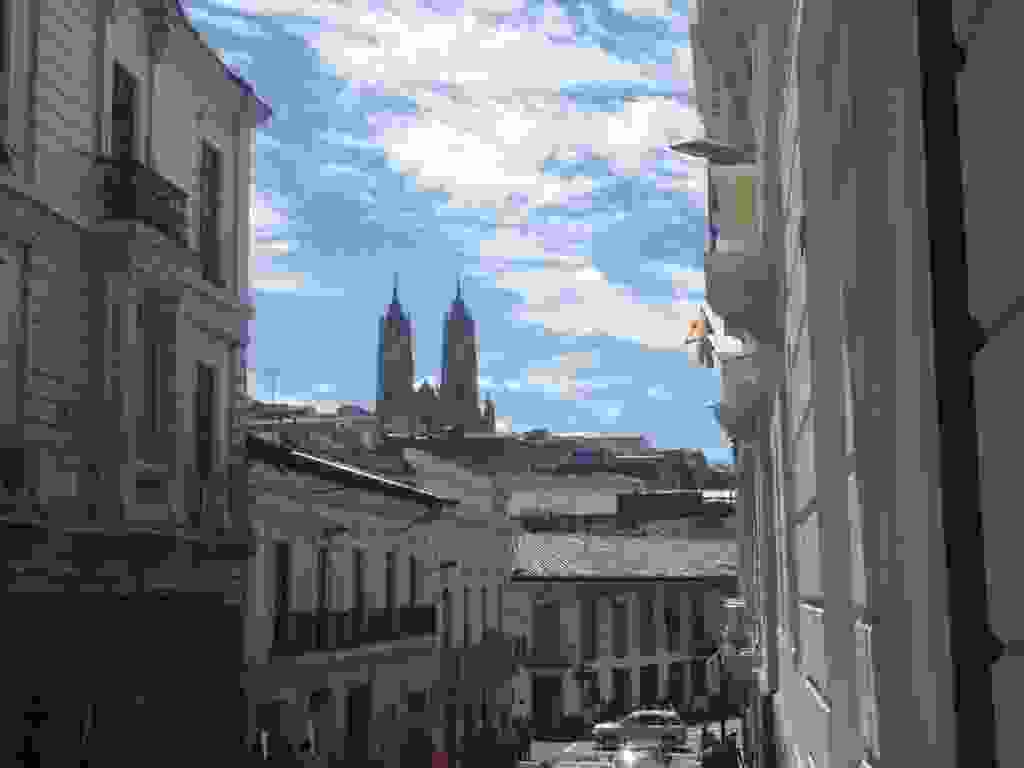
\includegraphics[height=90mm]{../wp-content/uploads/2015/06/P6305155-1024x768.jpg} } 
 \newline
 \newline
\centerline{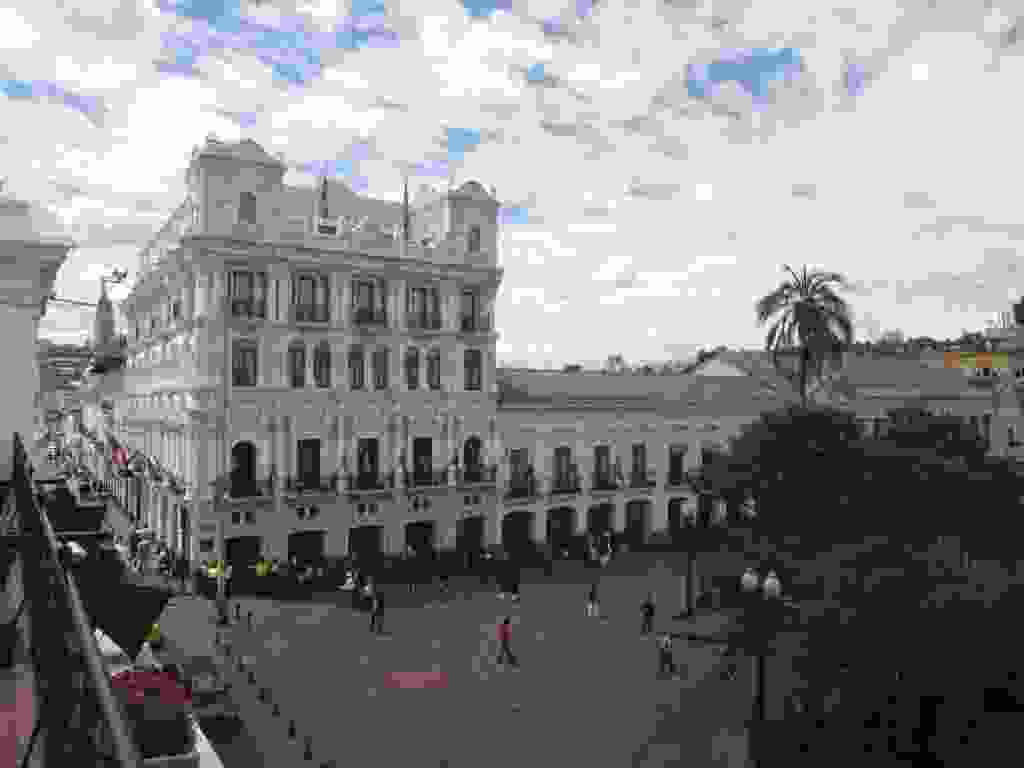
\includegraphics[height=90mm]{../wp-content/uploads/2015/06/P6305170-1024x768.jpg} } 
 \newline
 \newline
\centerline{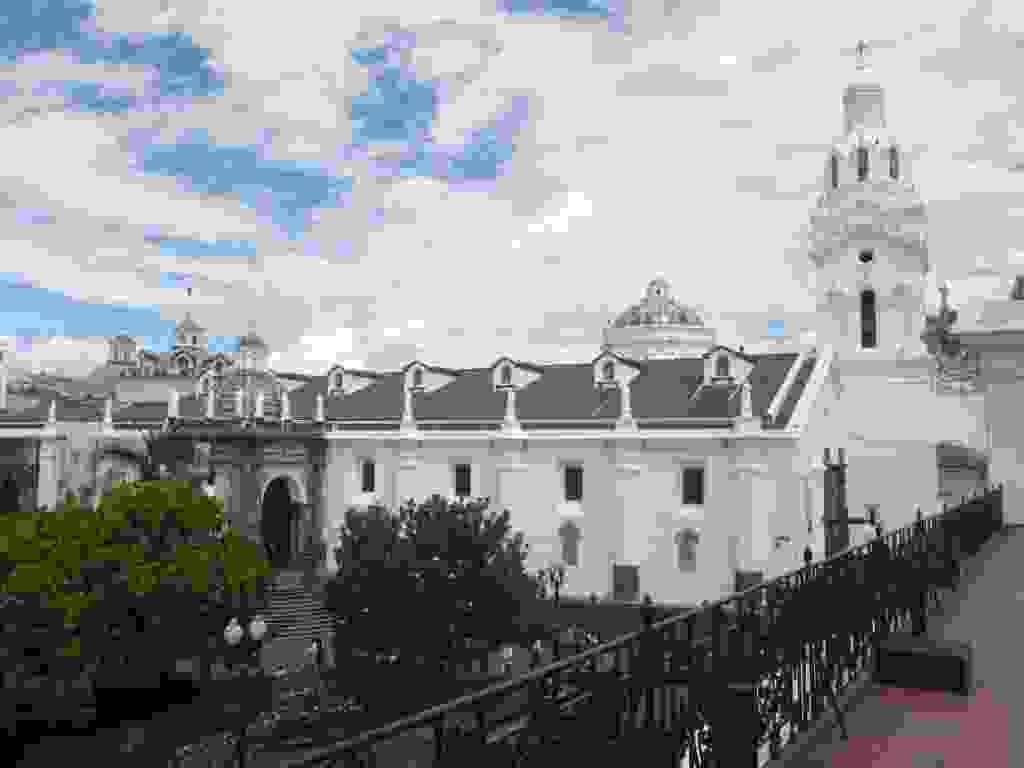
\includegraphics[height=90mm]{../wp-content/uploads/2015/06/P6305171-1024x768.jpg} } 
 \newline
 Il y a des dizaines, peut etre des centaines d´églises. \newline
 \newline
\centerline{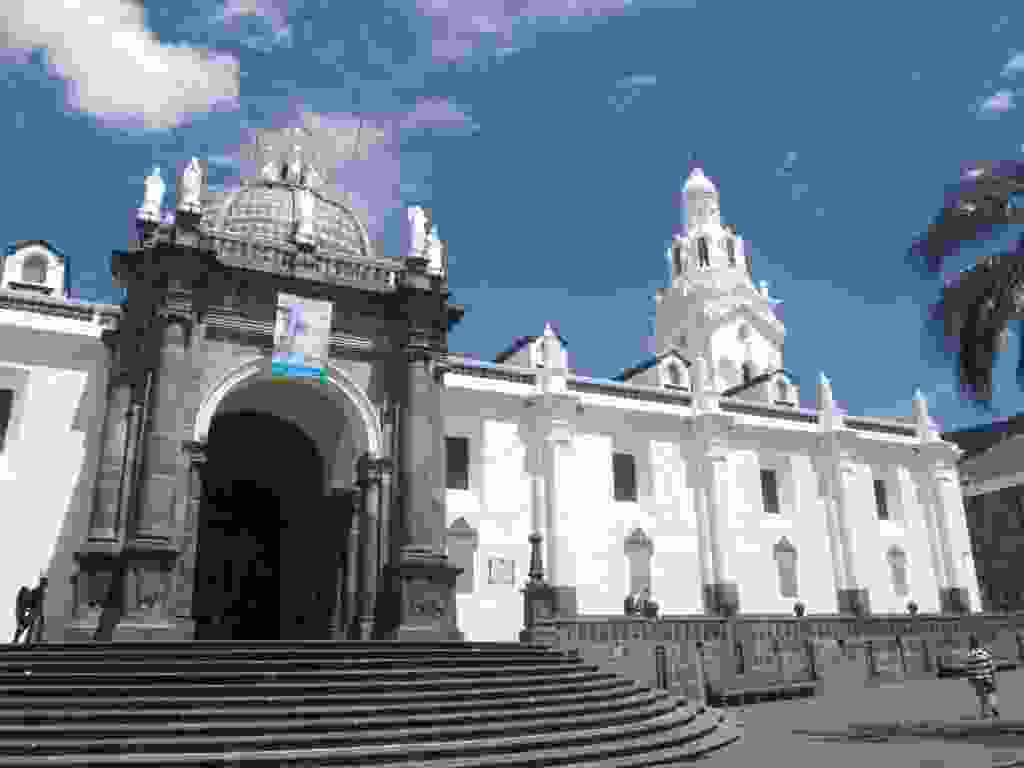
\includegraphics[height=90mm]{../wp-content/uploads/2015/06/P6305161-1024x768.jpg} } 
 \newline
 L'église Compania de Jesus dont l'intérieur est recouvert d'or. \newline
 \newline
\centerline{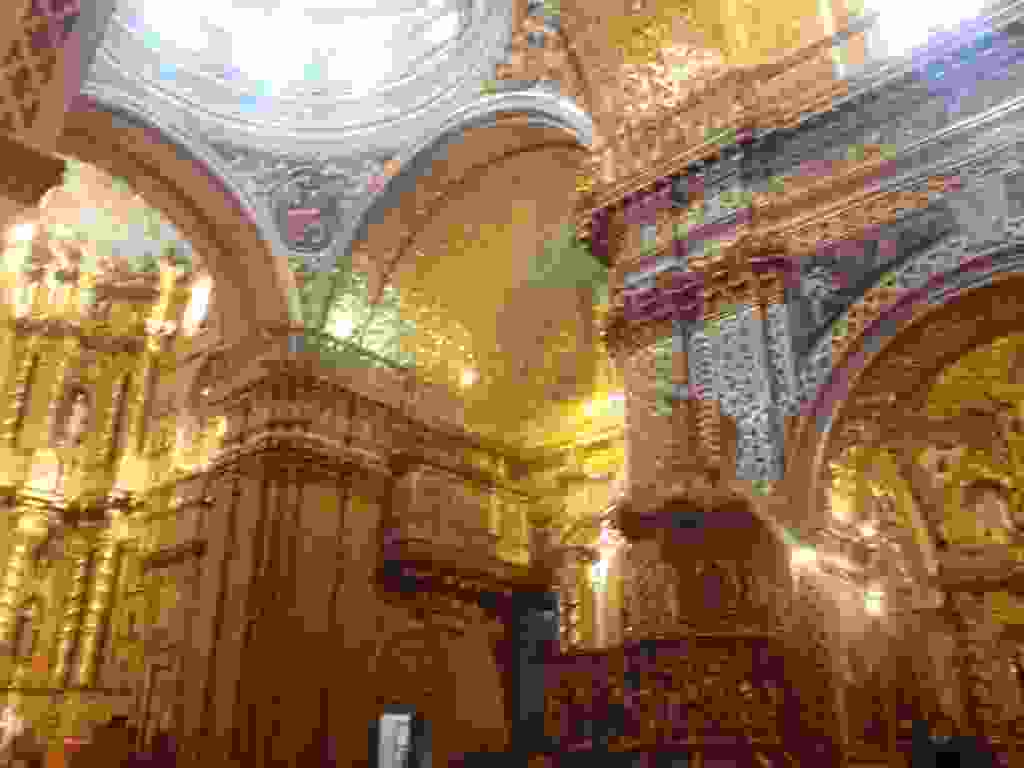
\includegraphics[height=90mm]{../wp-content/uploads/2015/06/P6275121-1024x768.jpg} } 
 \newline
 La basilique gothique. \newline
 \newline
\centerline{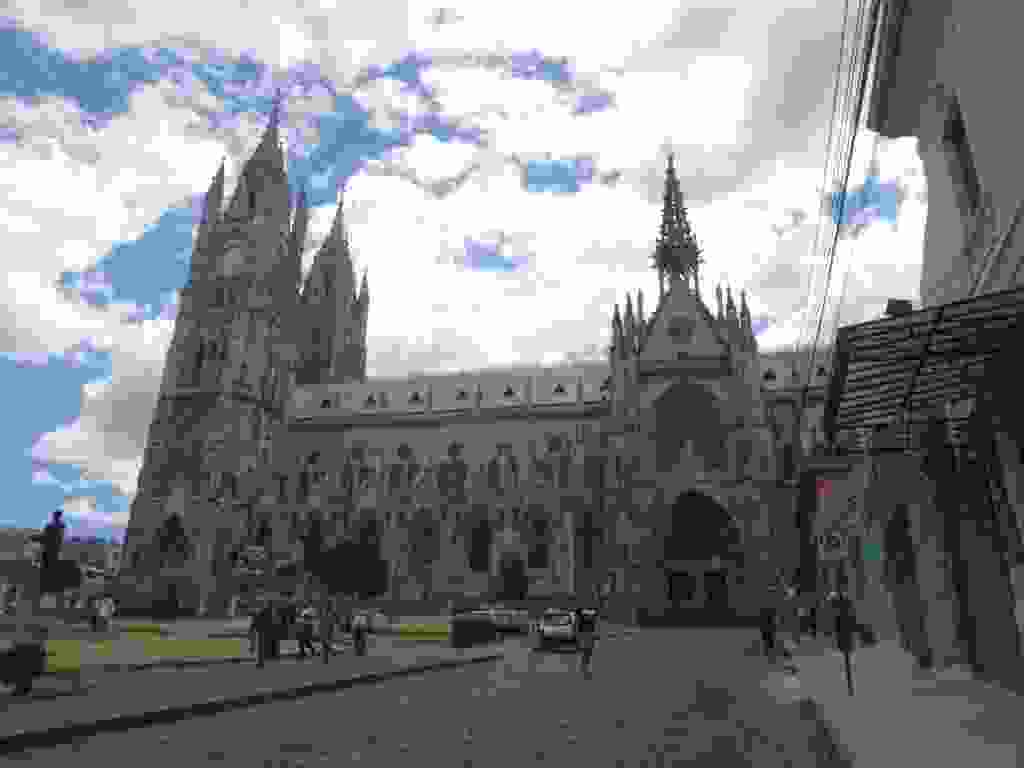
\includegraphics[height=90mm]{../wp-content/uploads/2015/06/P6305185-1024x768.jpg} } 
 \newline
 Le palais présidentiel ouvert au public gratuitement. \newline
 \newline
\centerline{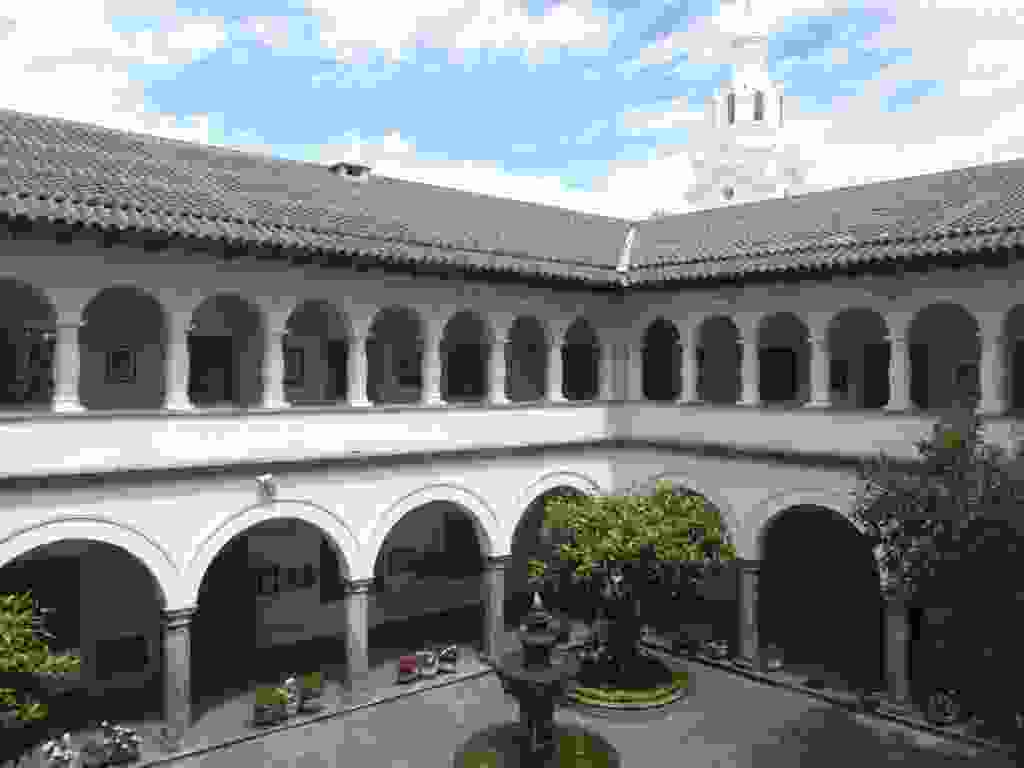
\includegraphics[height=90mm]{../wp-content/uploads/2015/06/P6305183-1024x768.jpg} } 
 \newline
 On peut visiter différentes salles et voir les cadeaux fait au président équatorien par des présidents étrangers. \newline
 \newline
\centerline{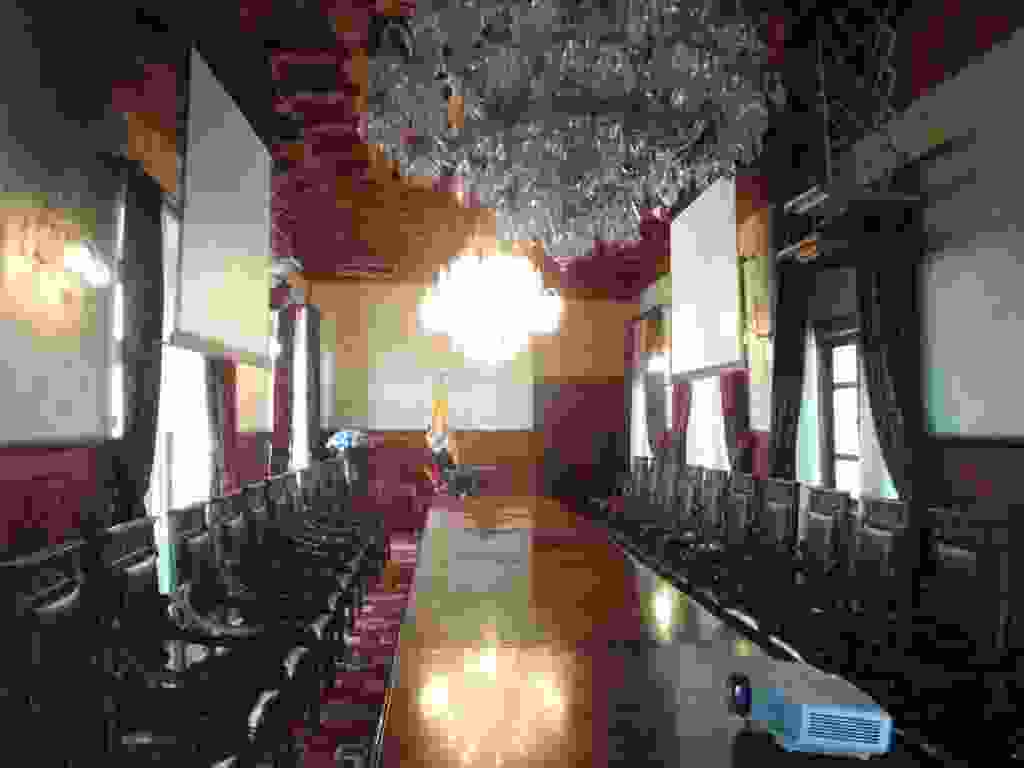
\includegraphics[height=90mm]{../wp-content/uploads/2015/06/P6305168-1024x768.jpg} } 
 \newline
 \newline
\centerline{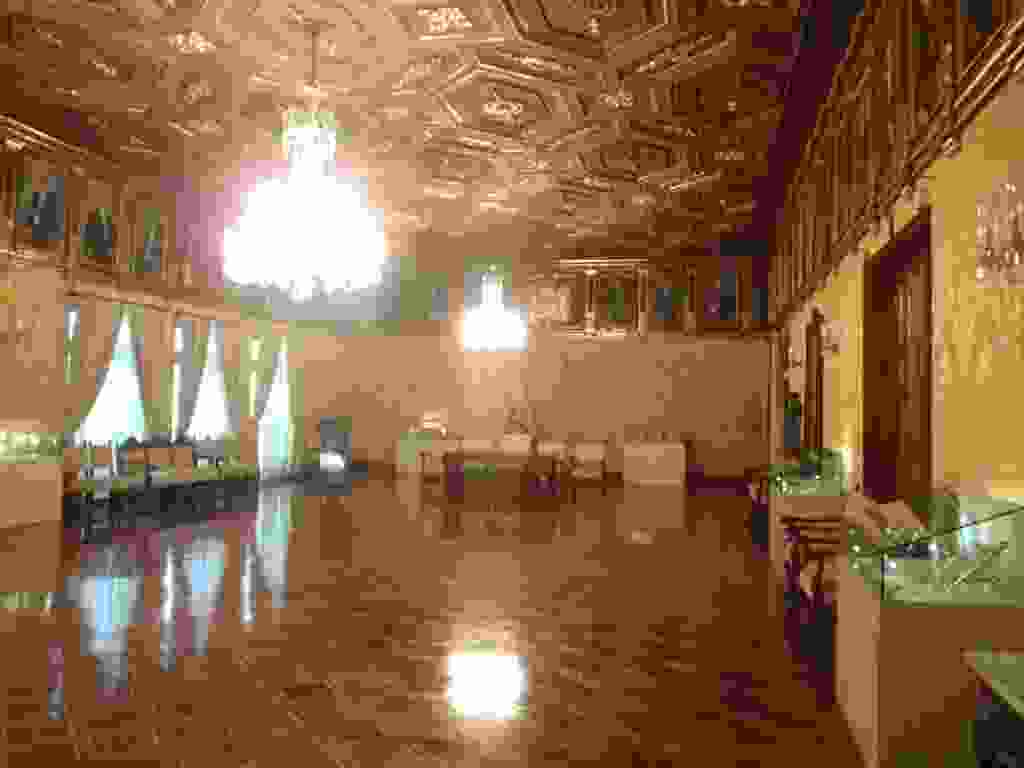
\includegraphics[height=90mm]{../wp-content/uploads/2015/06/P6305179-1024x768.jpg} } 
 \newline
 \newline
\centerline{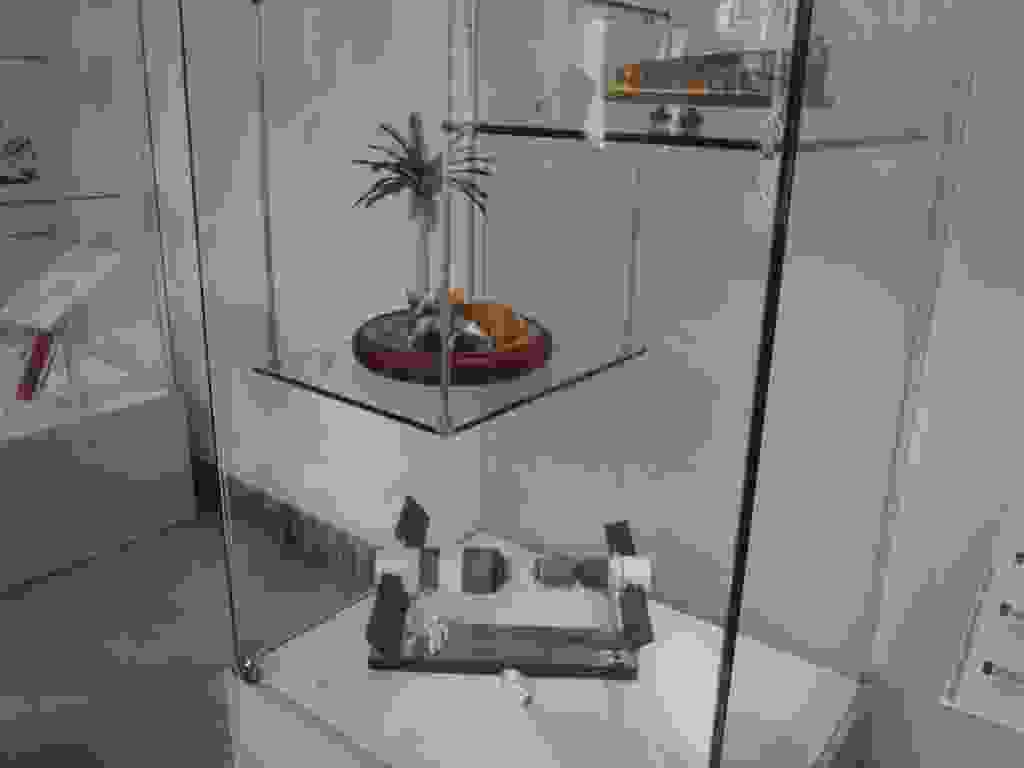
\includegraphics[height=90mm]{../wp-content/uploads/2015/06/P6305177-1024x768.jpg} } 
 \newline
 Avant de m´envoler vers les Galapagos, j´ai passé 2 jours dans une ferme à Pifo, un village pres de Quito. \newline
 4 familles s´y sont regroupées pour faire de l´élevage et du maraichage. \newline
 \newline
\centerline{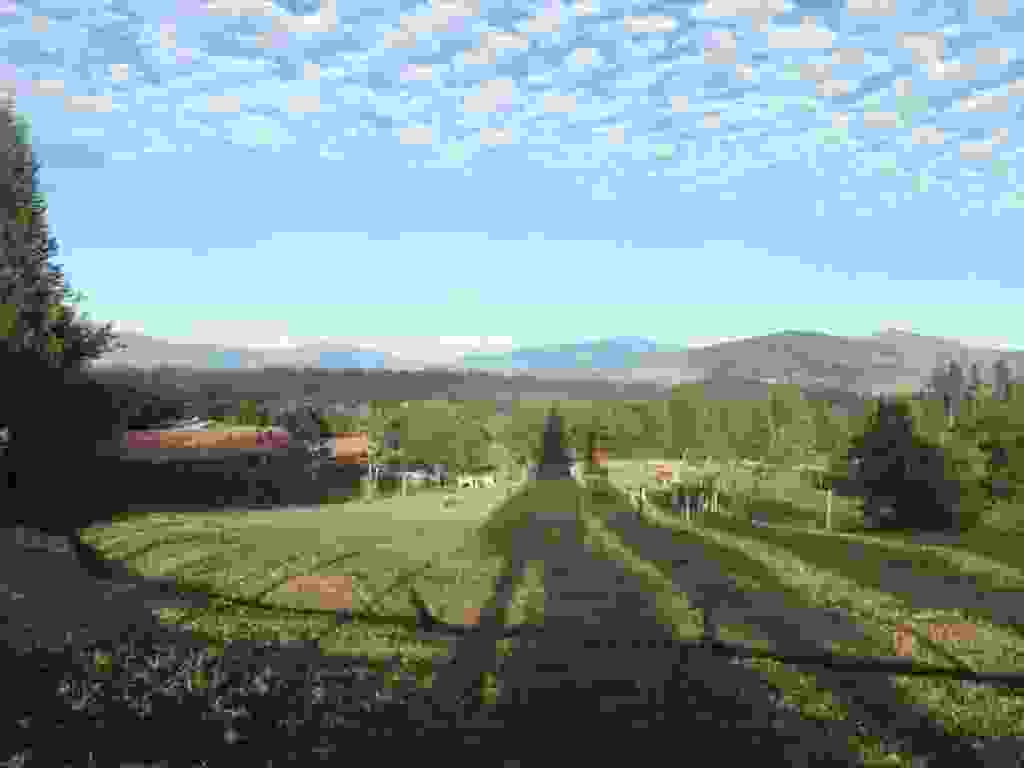
\includegraphics[height=90mm]{../wp-content/uploads/2015/06/P6305153-1024x768.jpg} } 
 \newline

\newpage
 
